\begin{center}
  \textbf{BAB IV} \\[0.5em]
  \textbf{HASIL DAN PEMBAHASAN}
\end{center}

\section*{4.1 Kebutuhan Hardware dan Software}
Hardware maupun Software yang digunakan dalam penelitian ini adalah sebagai berikut:

\begin{itemize}
  \item Hardware:
    \begin{itemize}
      \item CPU: M3
      \item RAM: 18 GB
      \item Storage: 512GB SSD
      \item VGA: M3 GPU
      \item Monitor: 15.6 inch Full HD
      \item Mouse: Wireless
      \item Keyboard: Wireless
    \end{itemize}
  \item Software:
    \begin{itemize}
      \item Operating System: MacOS Sequoia 15.3.2
      \item IDE: Vs Code, Cursor
      \item Database: PostgreSQL
      \item Framework: Laravel
      \item Programming Language: PHP, JavaScript, HTML, CSS, SQL
    \end{itemize}
\end{itemize}

\section*{4.2 Implementasi}

Langkah berikutnya setelah melakukan perancangan sistem adalah implementasi sistem dalam pengkodean. 
Berikut adalah hasil implementasi dari sistem yang telah dirancang.

\subsection*{4.2.1 Tampilan UI Register}
halaman register digunakan untuk membuat akun baru pada sistem.
\begin{center}
  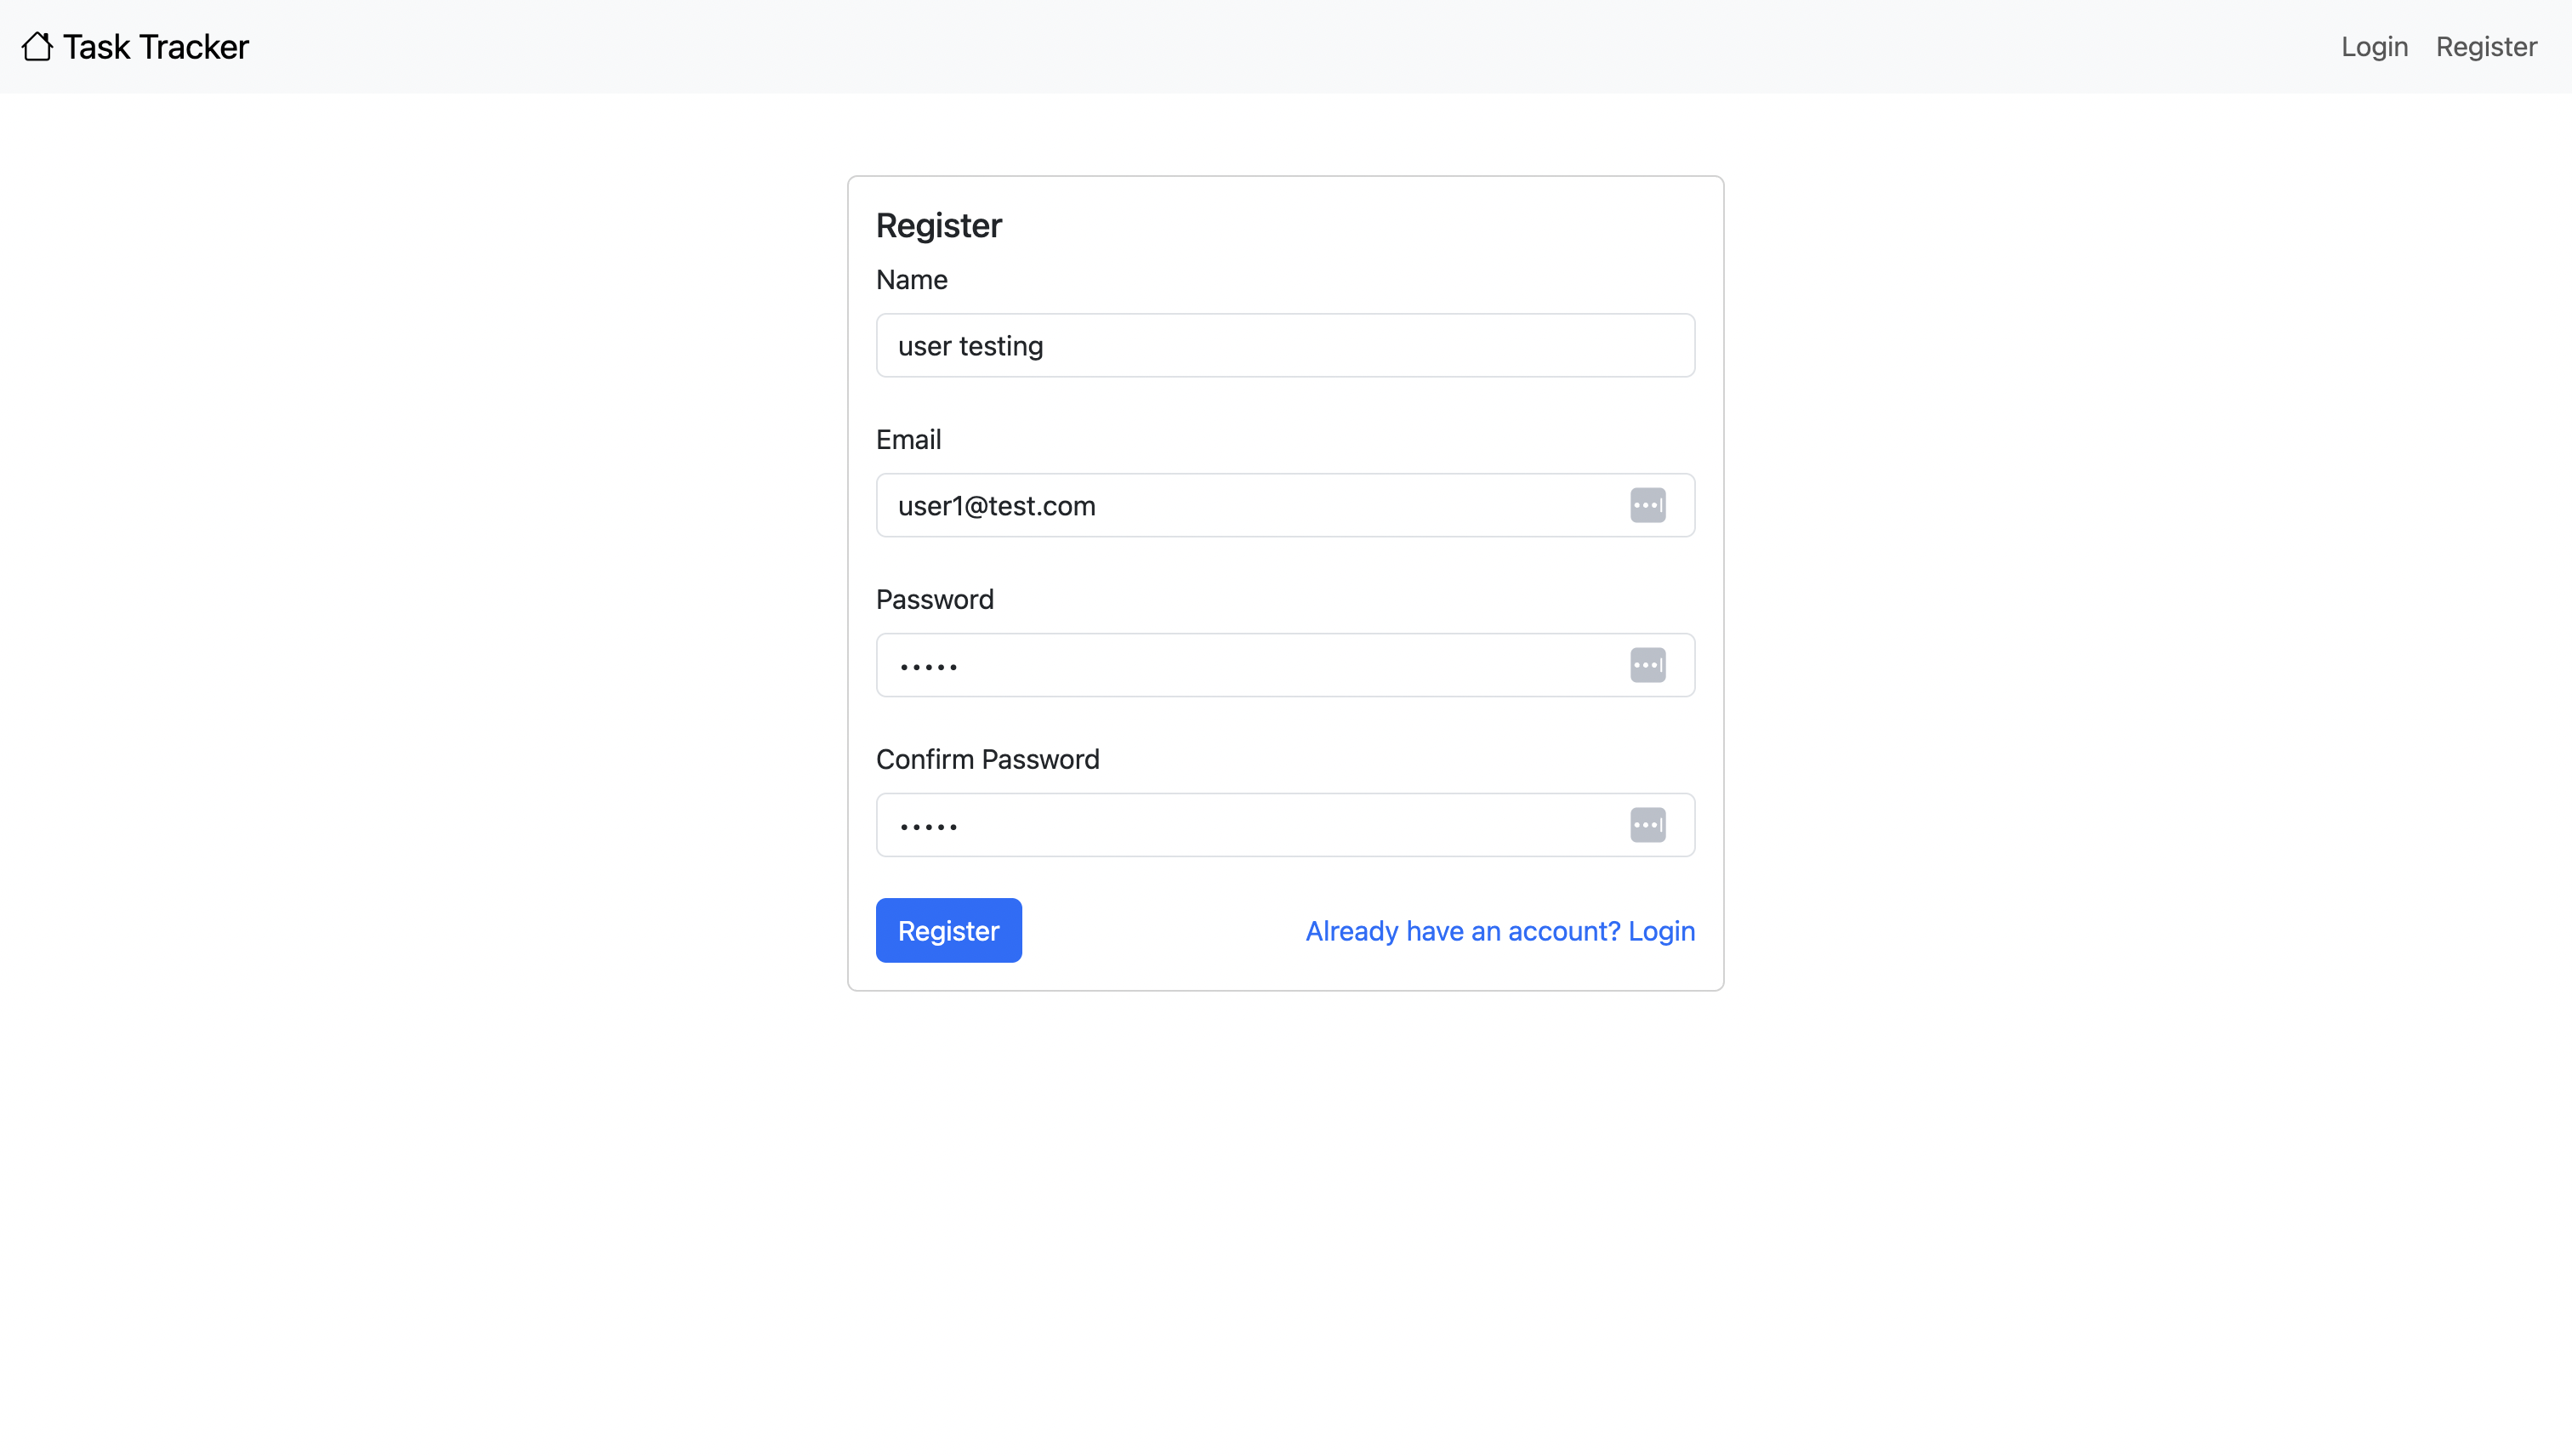
\includegraphics[width=1\textwidth]{assets/ui/register_filled.png}
  \captionof{figure}{Tampilan UI Register}
\end{center}


\subsection*{4.2.2 Tampilan UI Login}
halaman login digunakan untuk masuk ke dalam sistem.
\begin{center}
  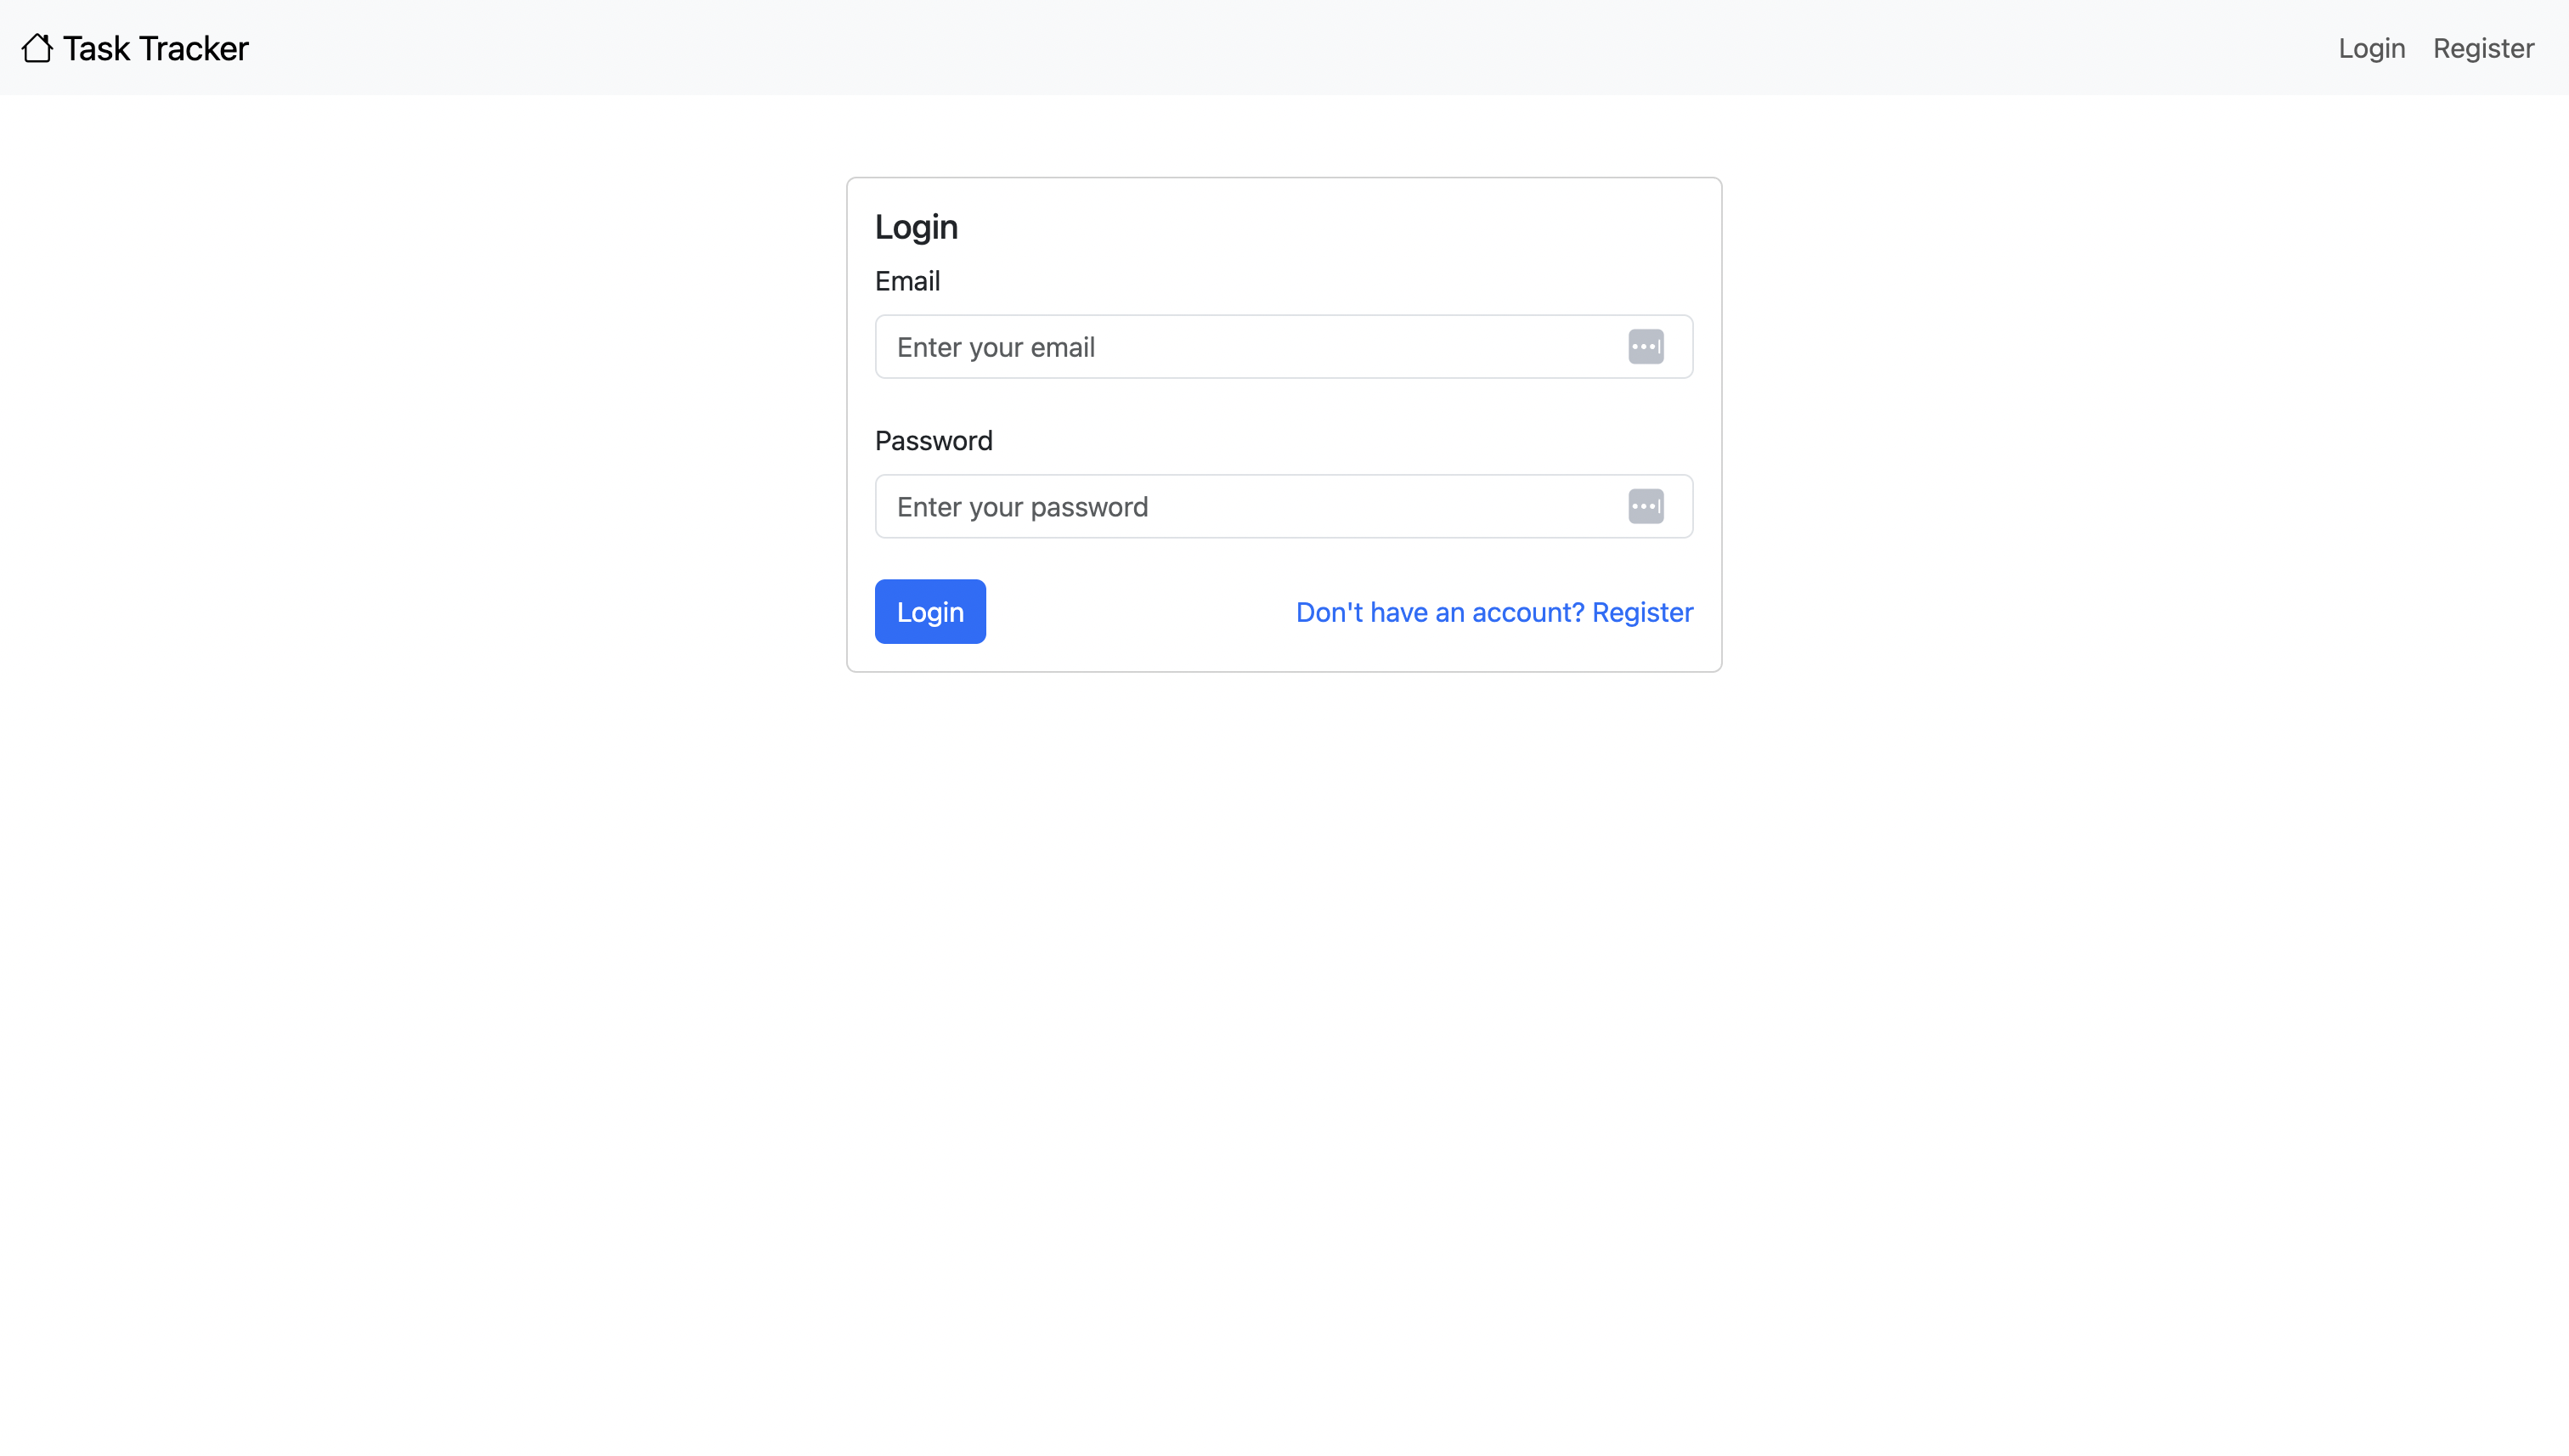
\includegraphics[width=1\textwidth]{assets/ui/login.png}
  \captionof{figure}{Tampilan UI Login}
\end{center}

\subsection*{4.2.3 Tampilan UI Dashboard}
halaman dashboard digunakan untuk menampilkan informasi terkait akun yang sedang login.
\begin{center}
  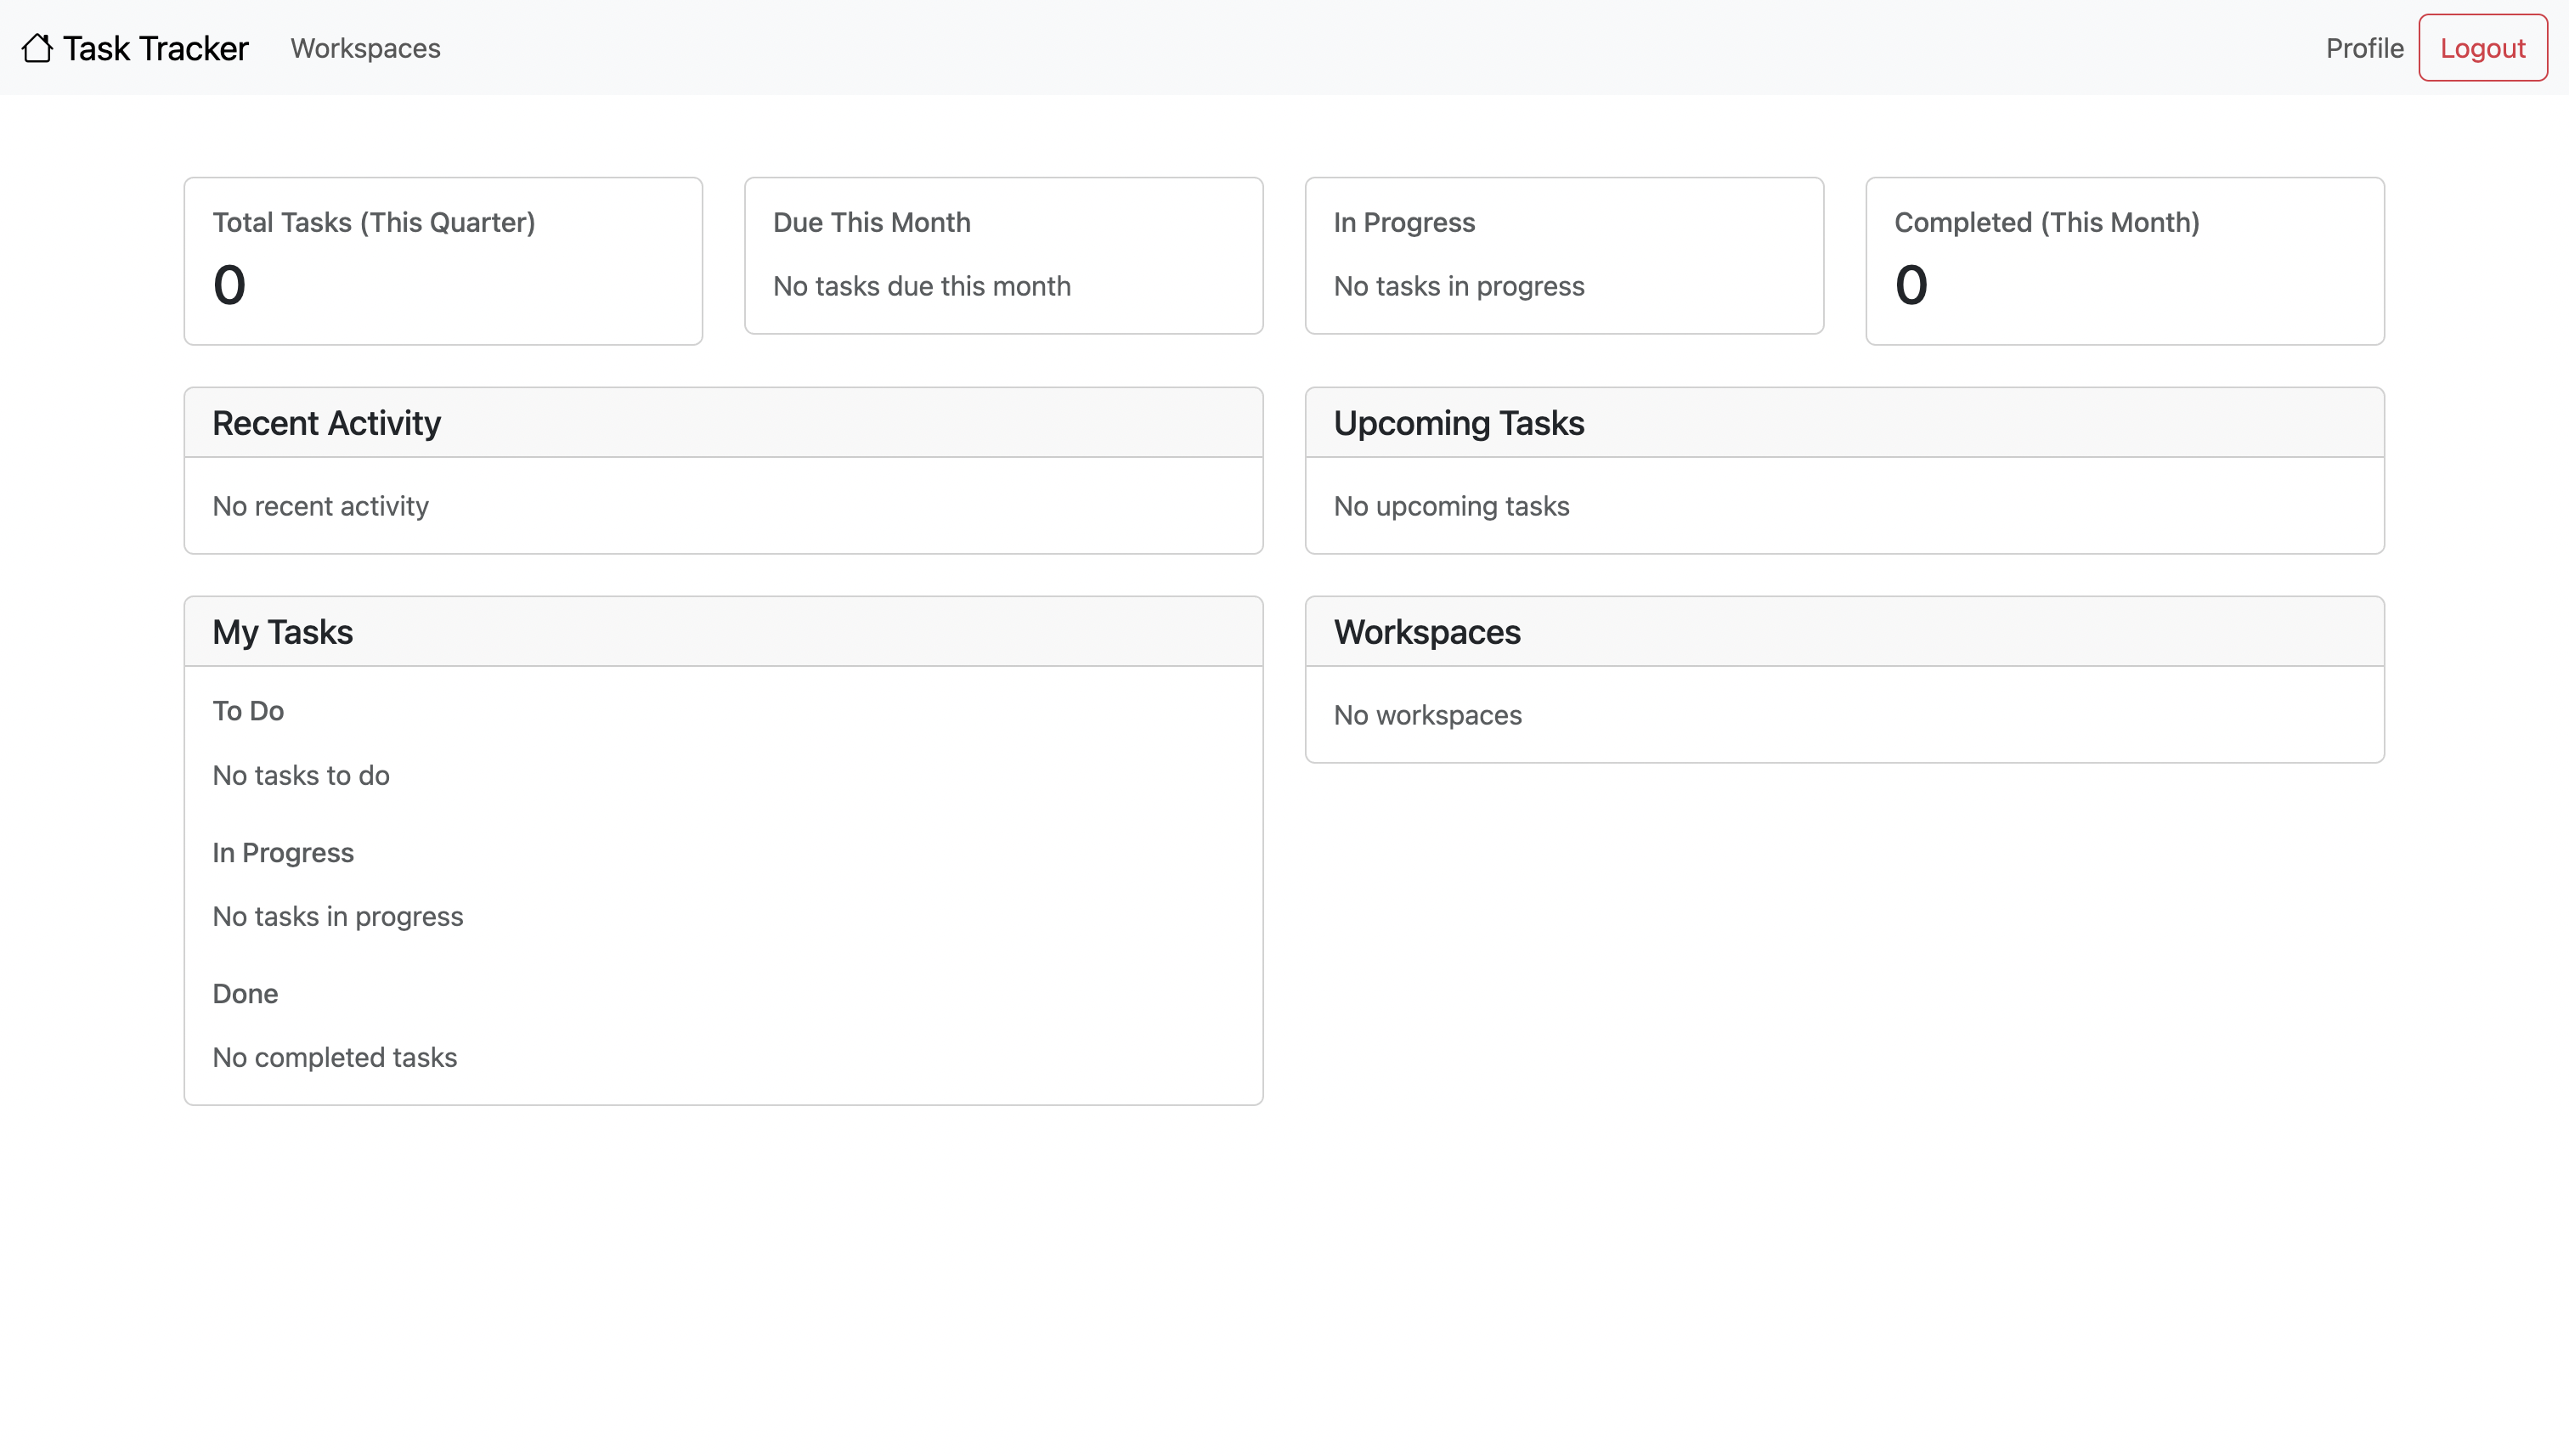
\includegraphics[width=1\textwidth]{assets/ui/empty_dashboard.png}
  \captionof{figure}{Tampilan UI Dashboard Kosong}
\end{center}
\begin{center}
  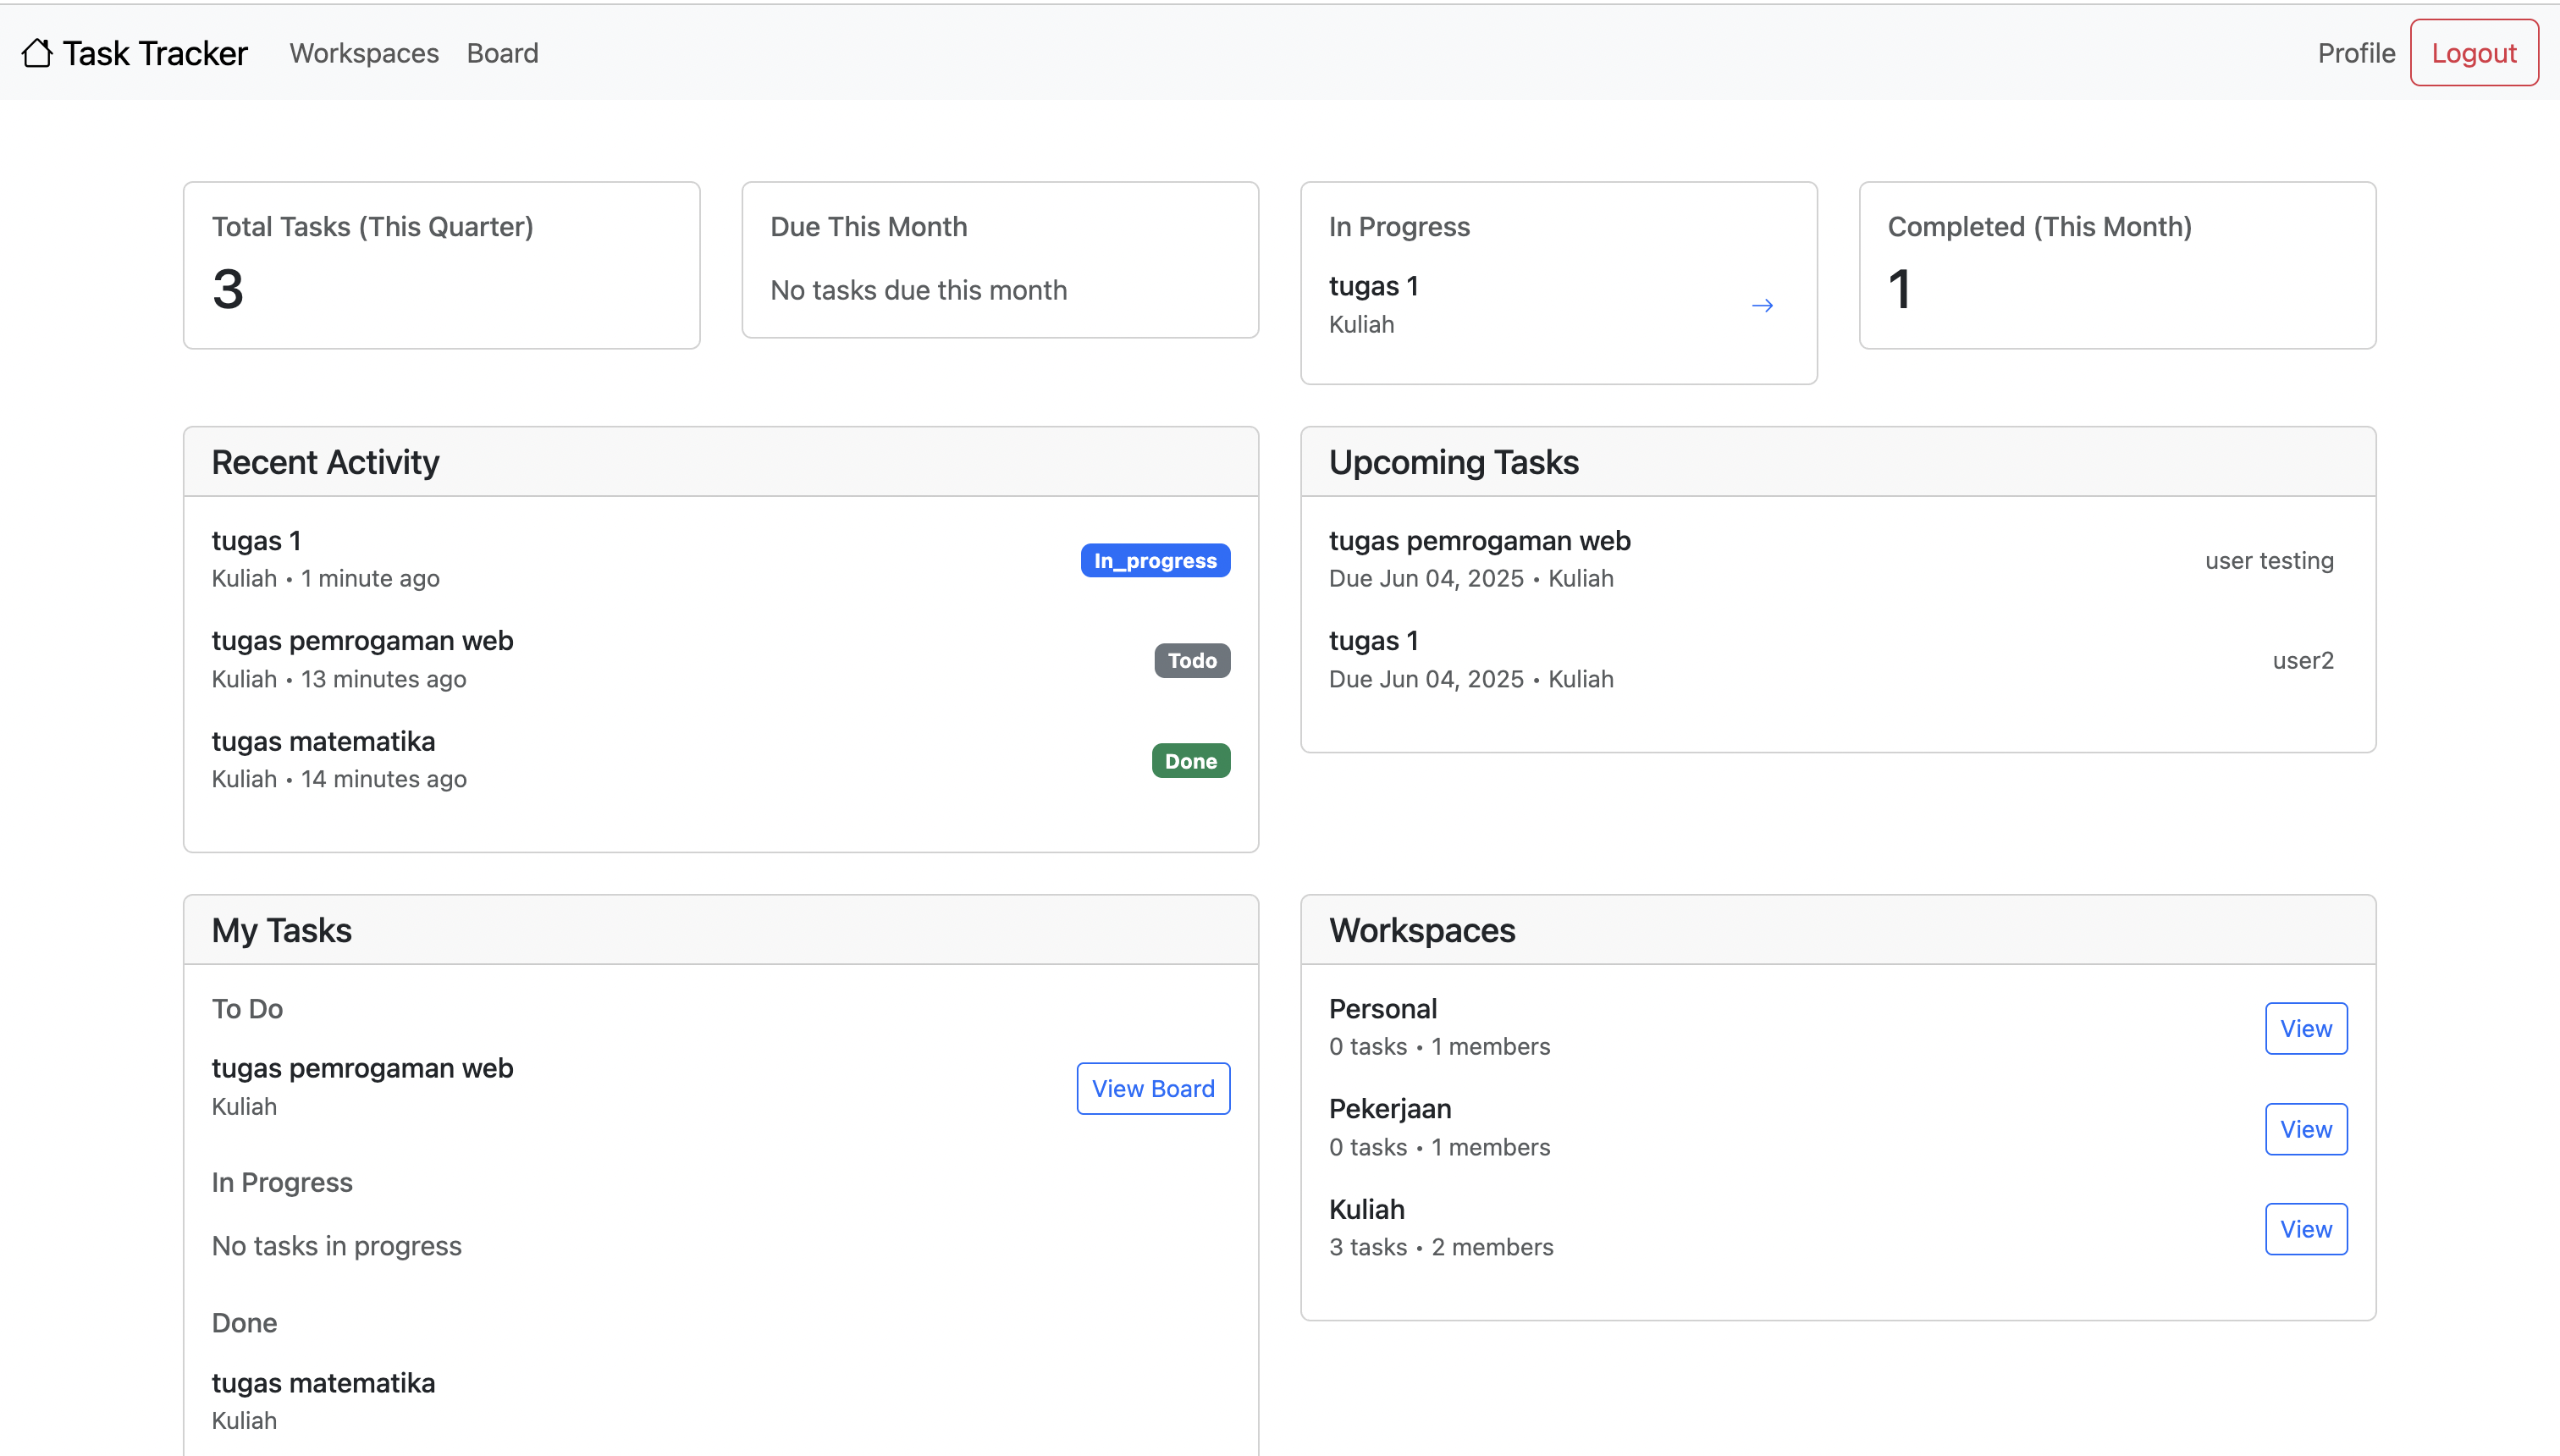
\includegraphics[width=1\textwidth]{assets/ui/user_dashboard_filled.png}
  \captionof{figure}{Tampilan UI Dashboard Terisi}
\end{center}

\subsection*{4.2.4 Tampilan UI Profile}
halaman profile digunakan untuk menampilkan informasi terkait akun yang sedang login.
halman ini juga digunakan untuk mengubah informasi akun yang sedang login, seperti nama dan password.
\begin{center}
  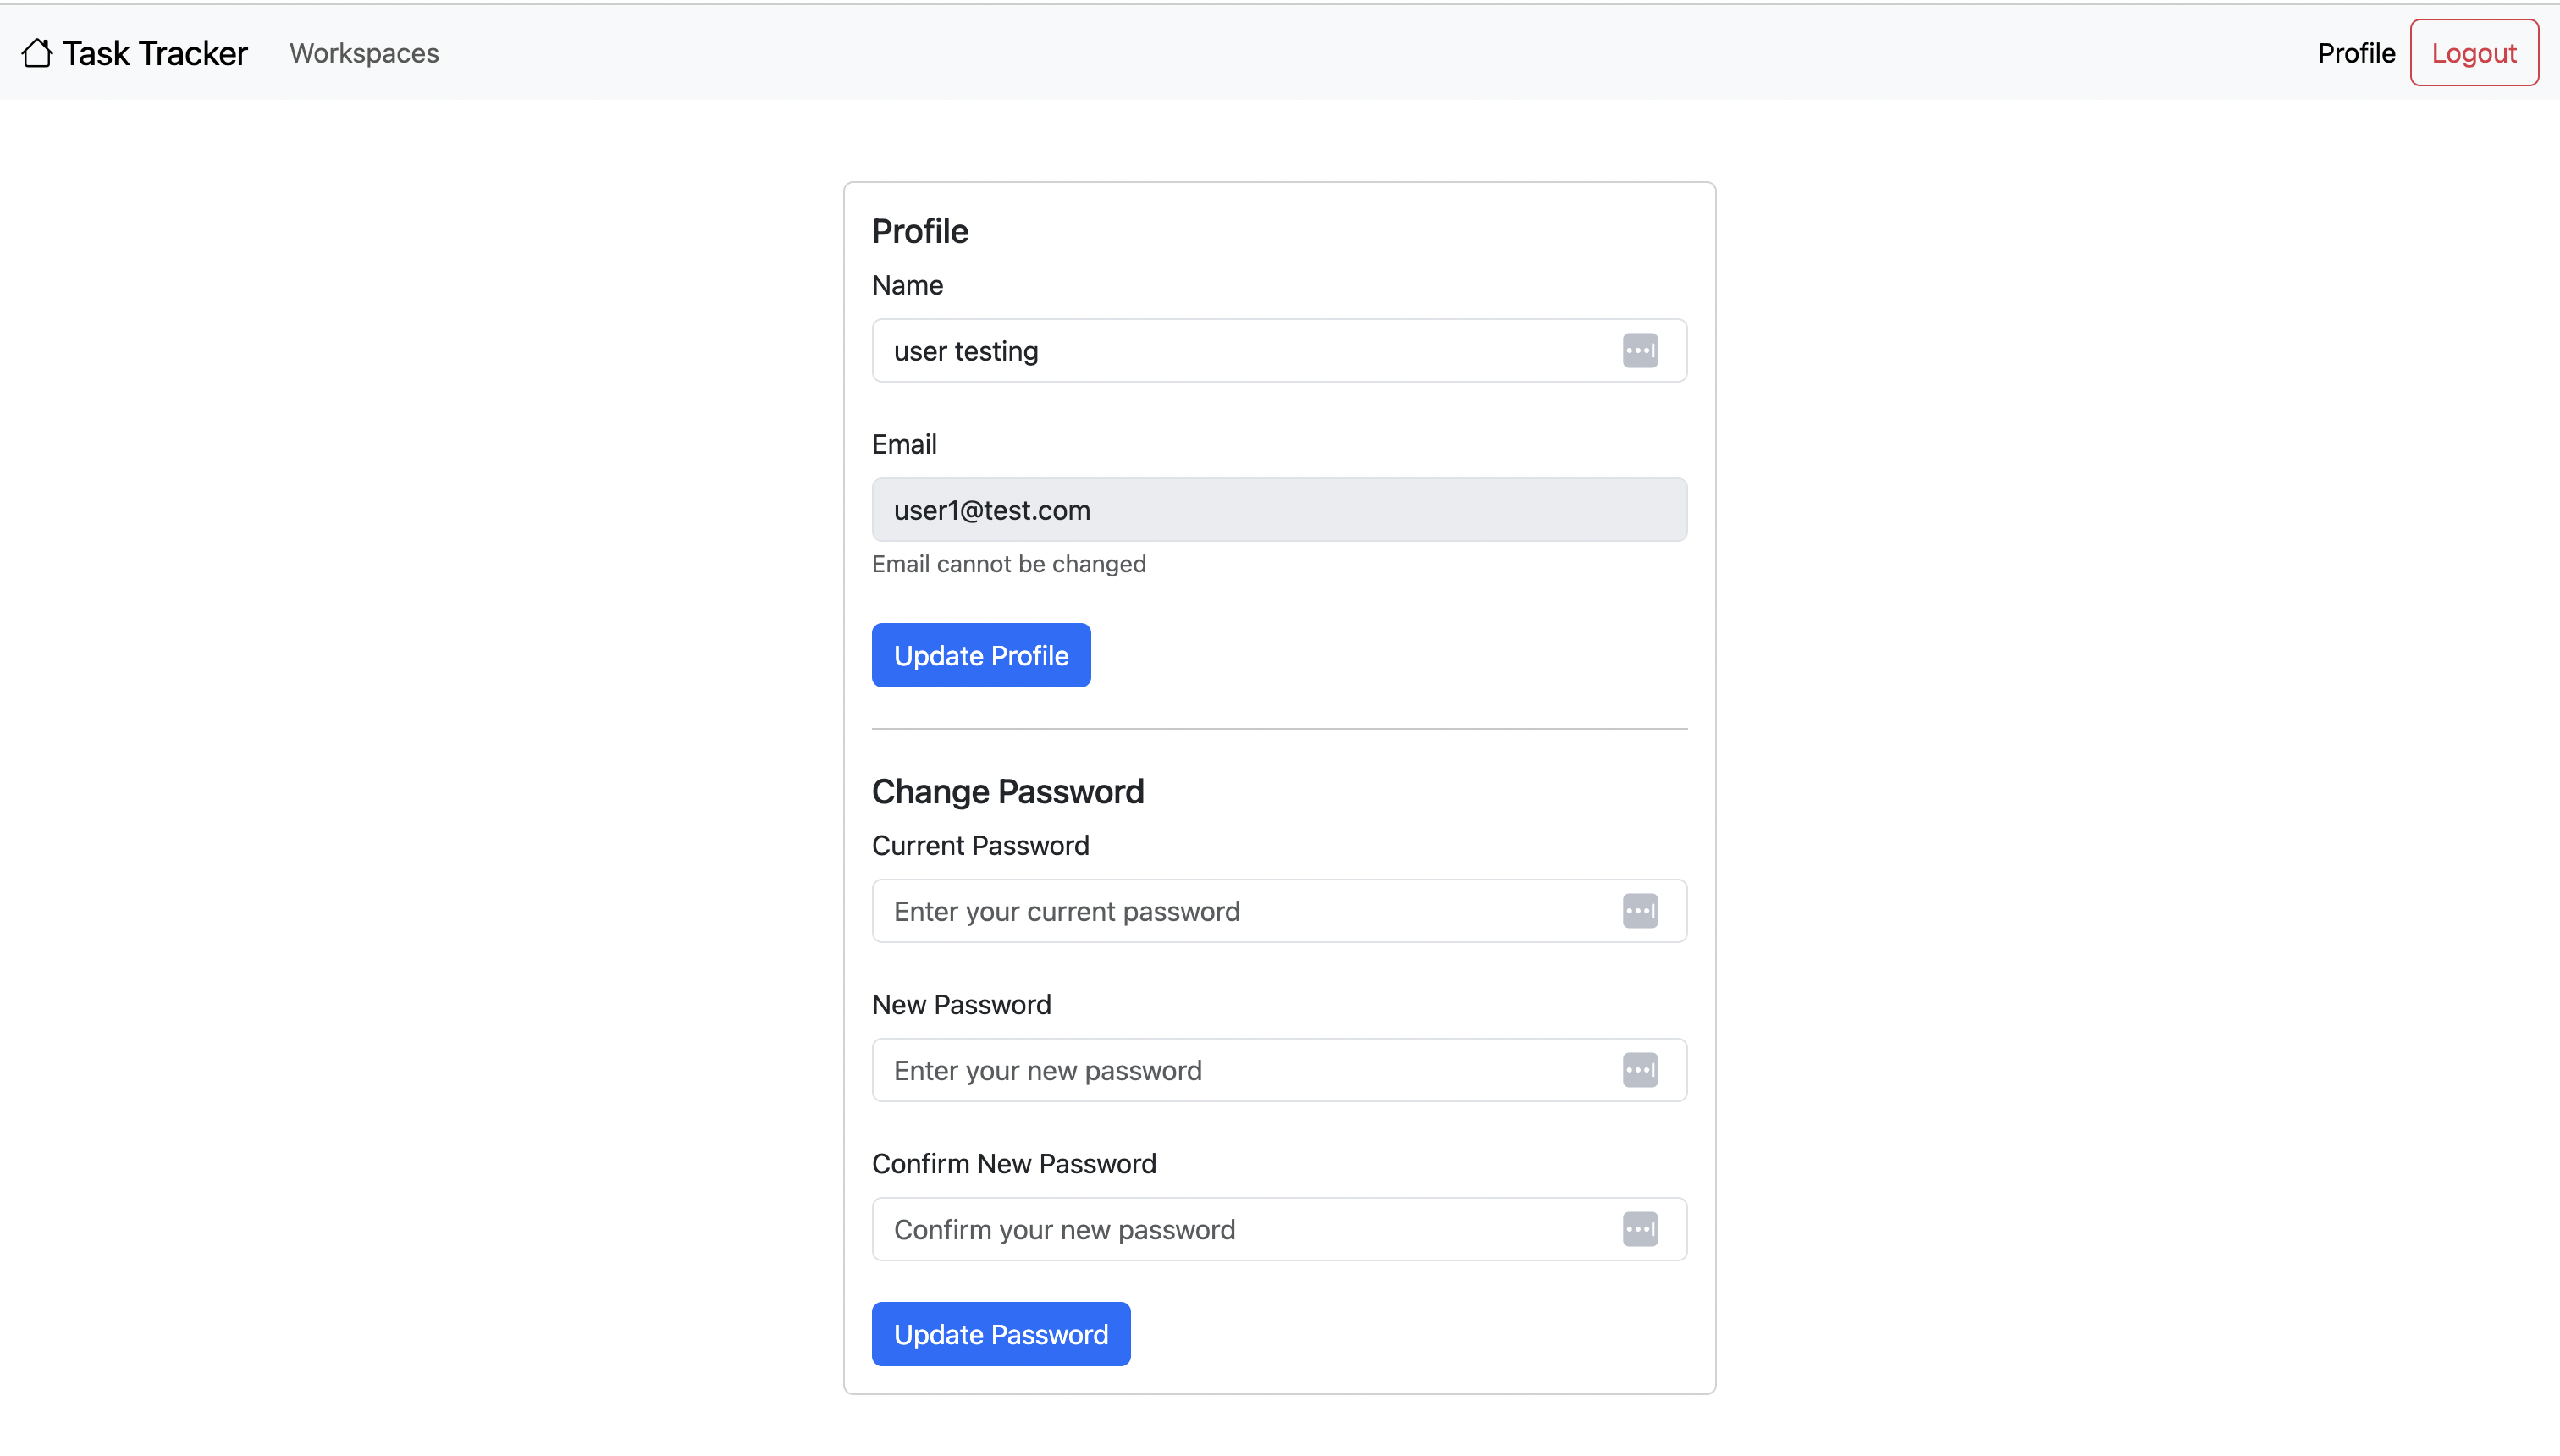
\includegraphics[width=1\textwidth]{assets/ui/edit_profile.png}
  \captionof{figure}{Tampilan UI Profile}
\end{center}



\subsection*{4.2.5 Tampilan UI Workspace}
halaman workspace digunakan untuk manajemen workspace. 
seperti membuat workspace baru, mengubah nama workspace, dan menghapus workspace.
\begin{center}
  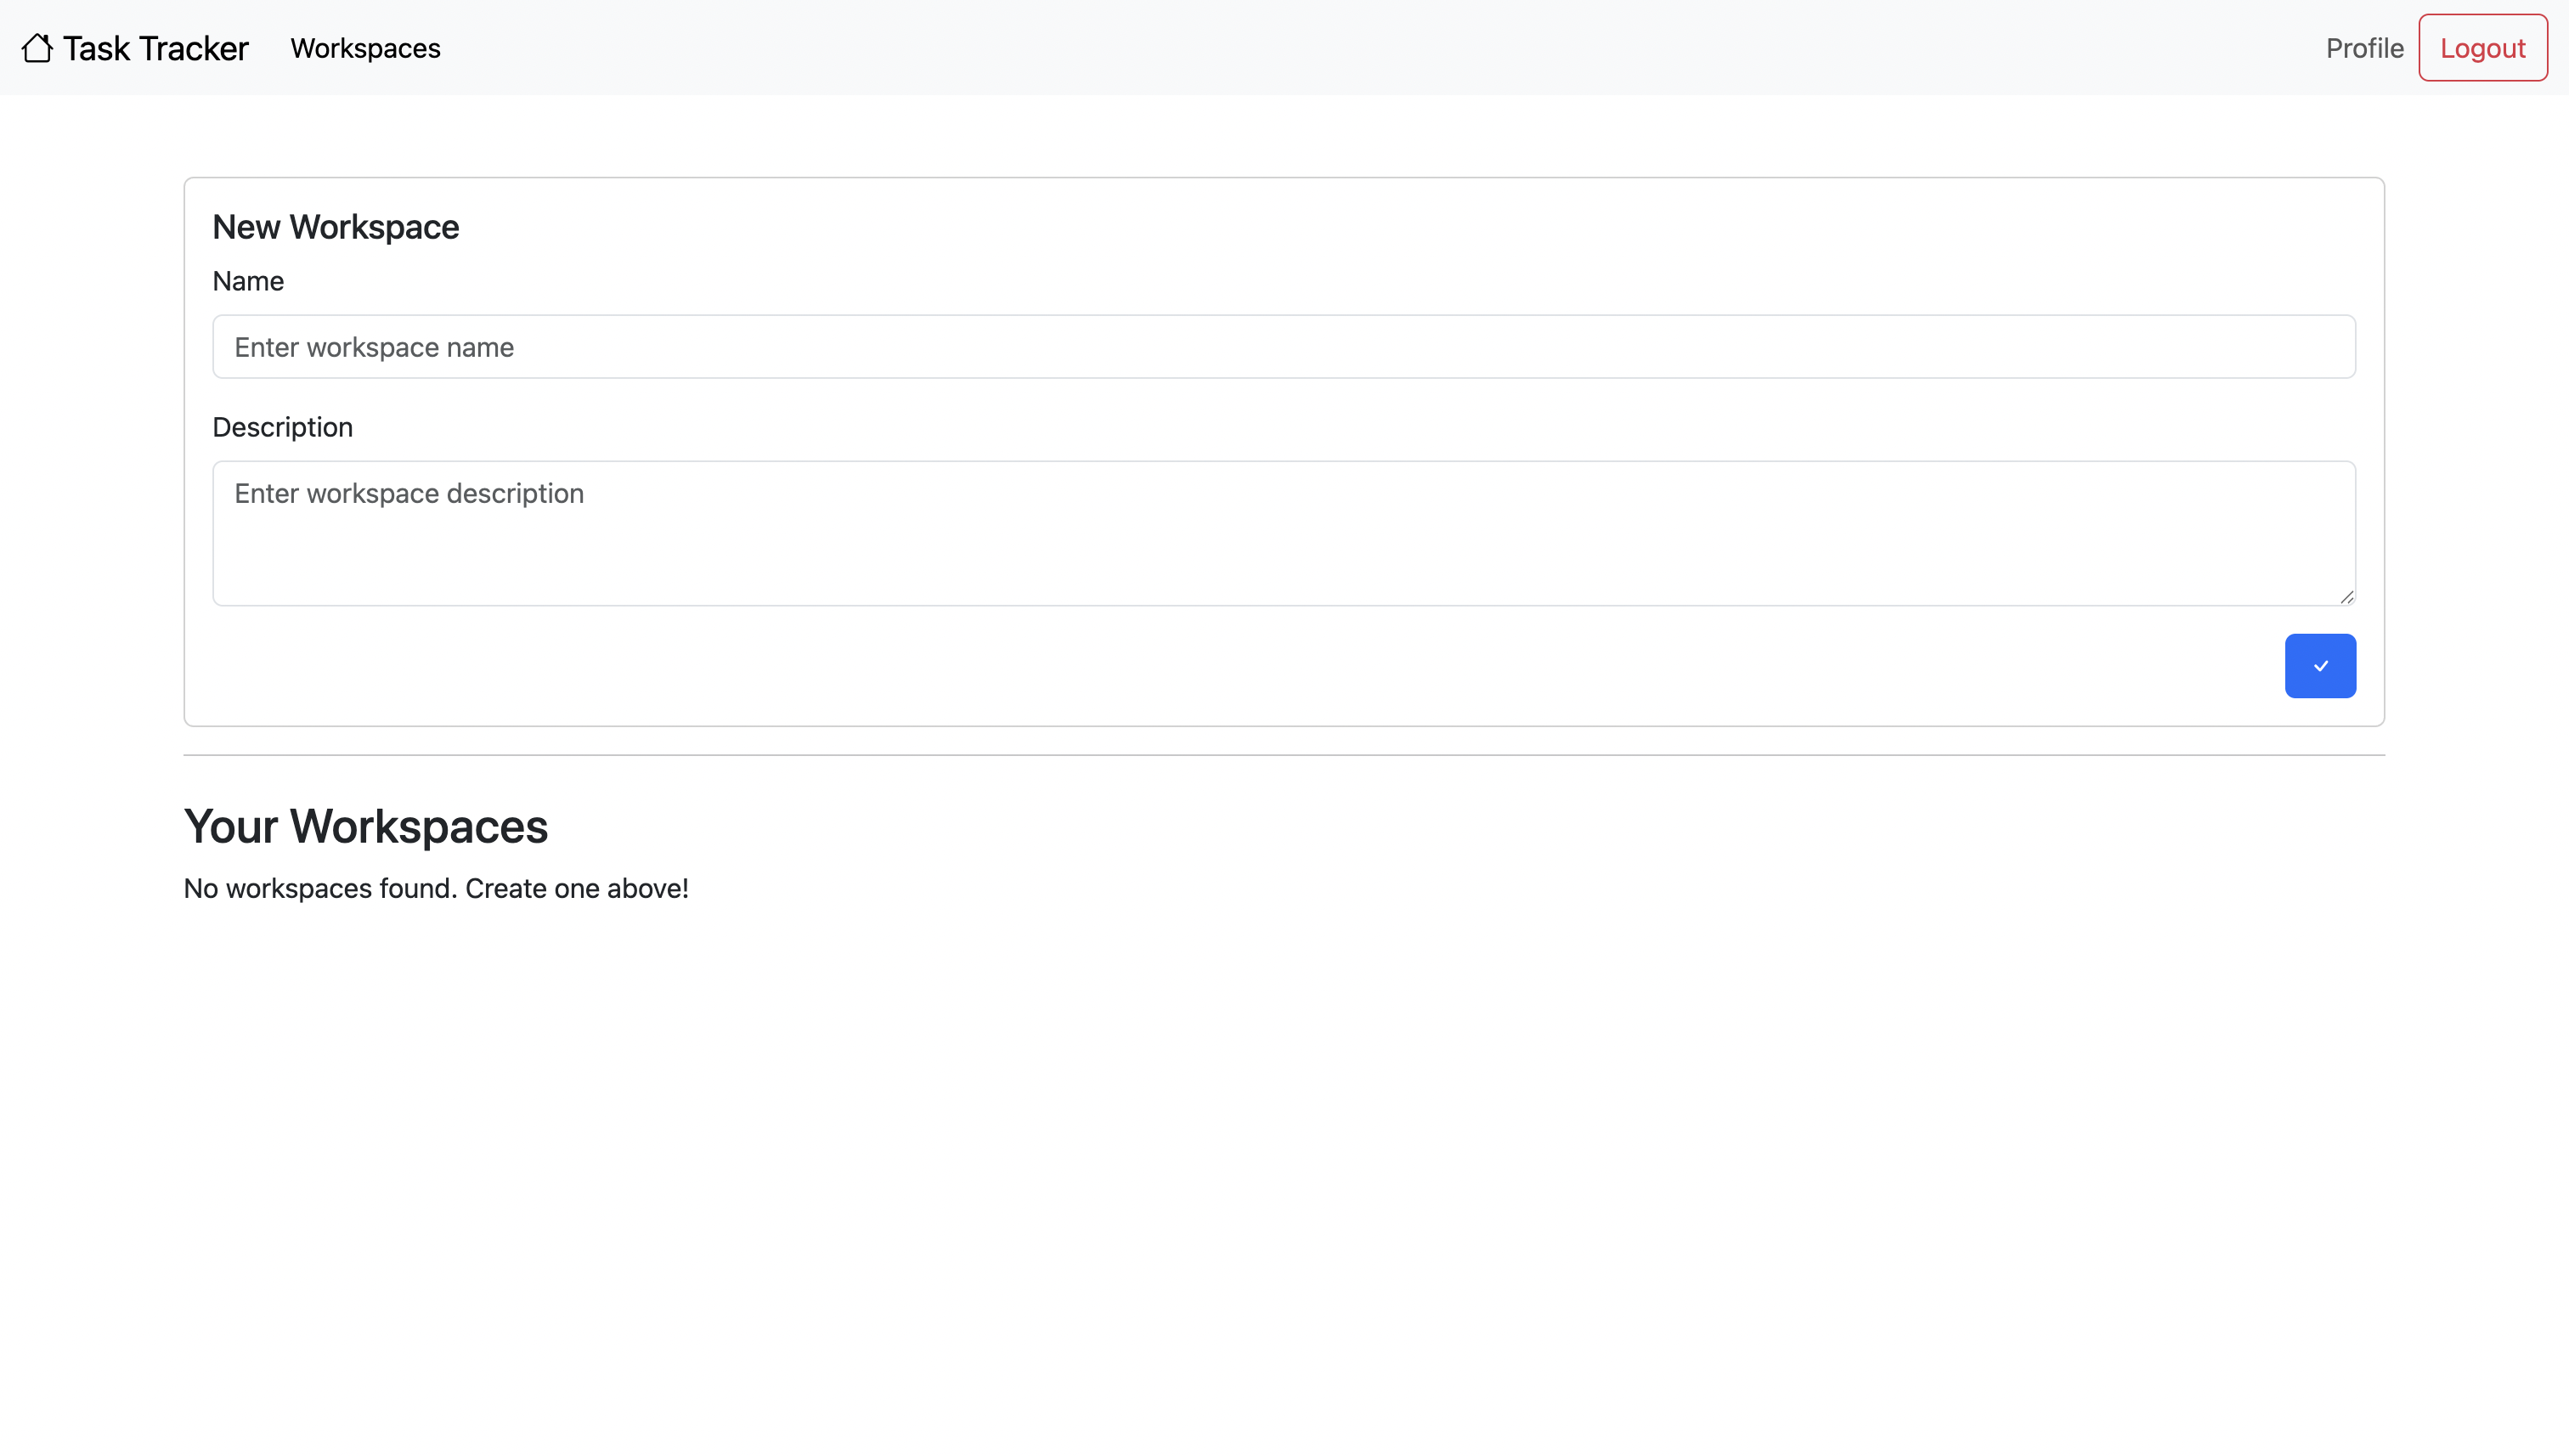
\includegraphics[width=1\textwidth]{assets/ui/workspace_empty.png}
  \captionof{figure}{Tampilan UI Workspace Kosong}
\end{center}
\begin{center}
  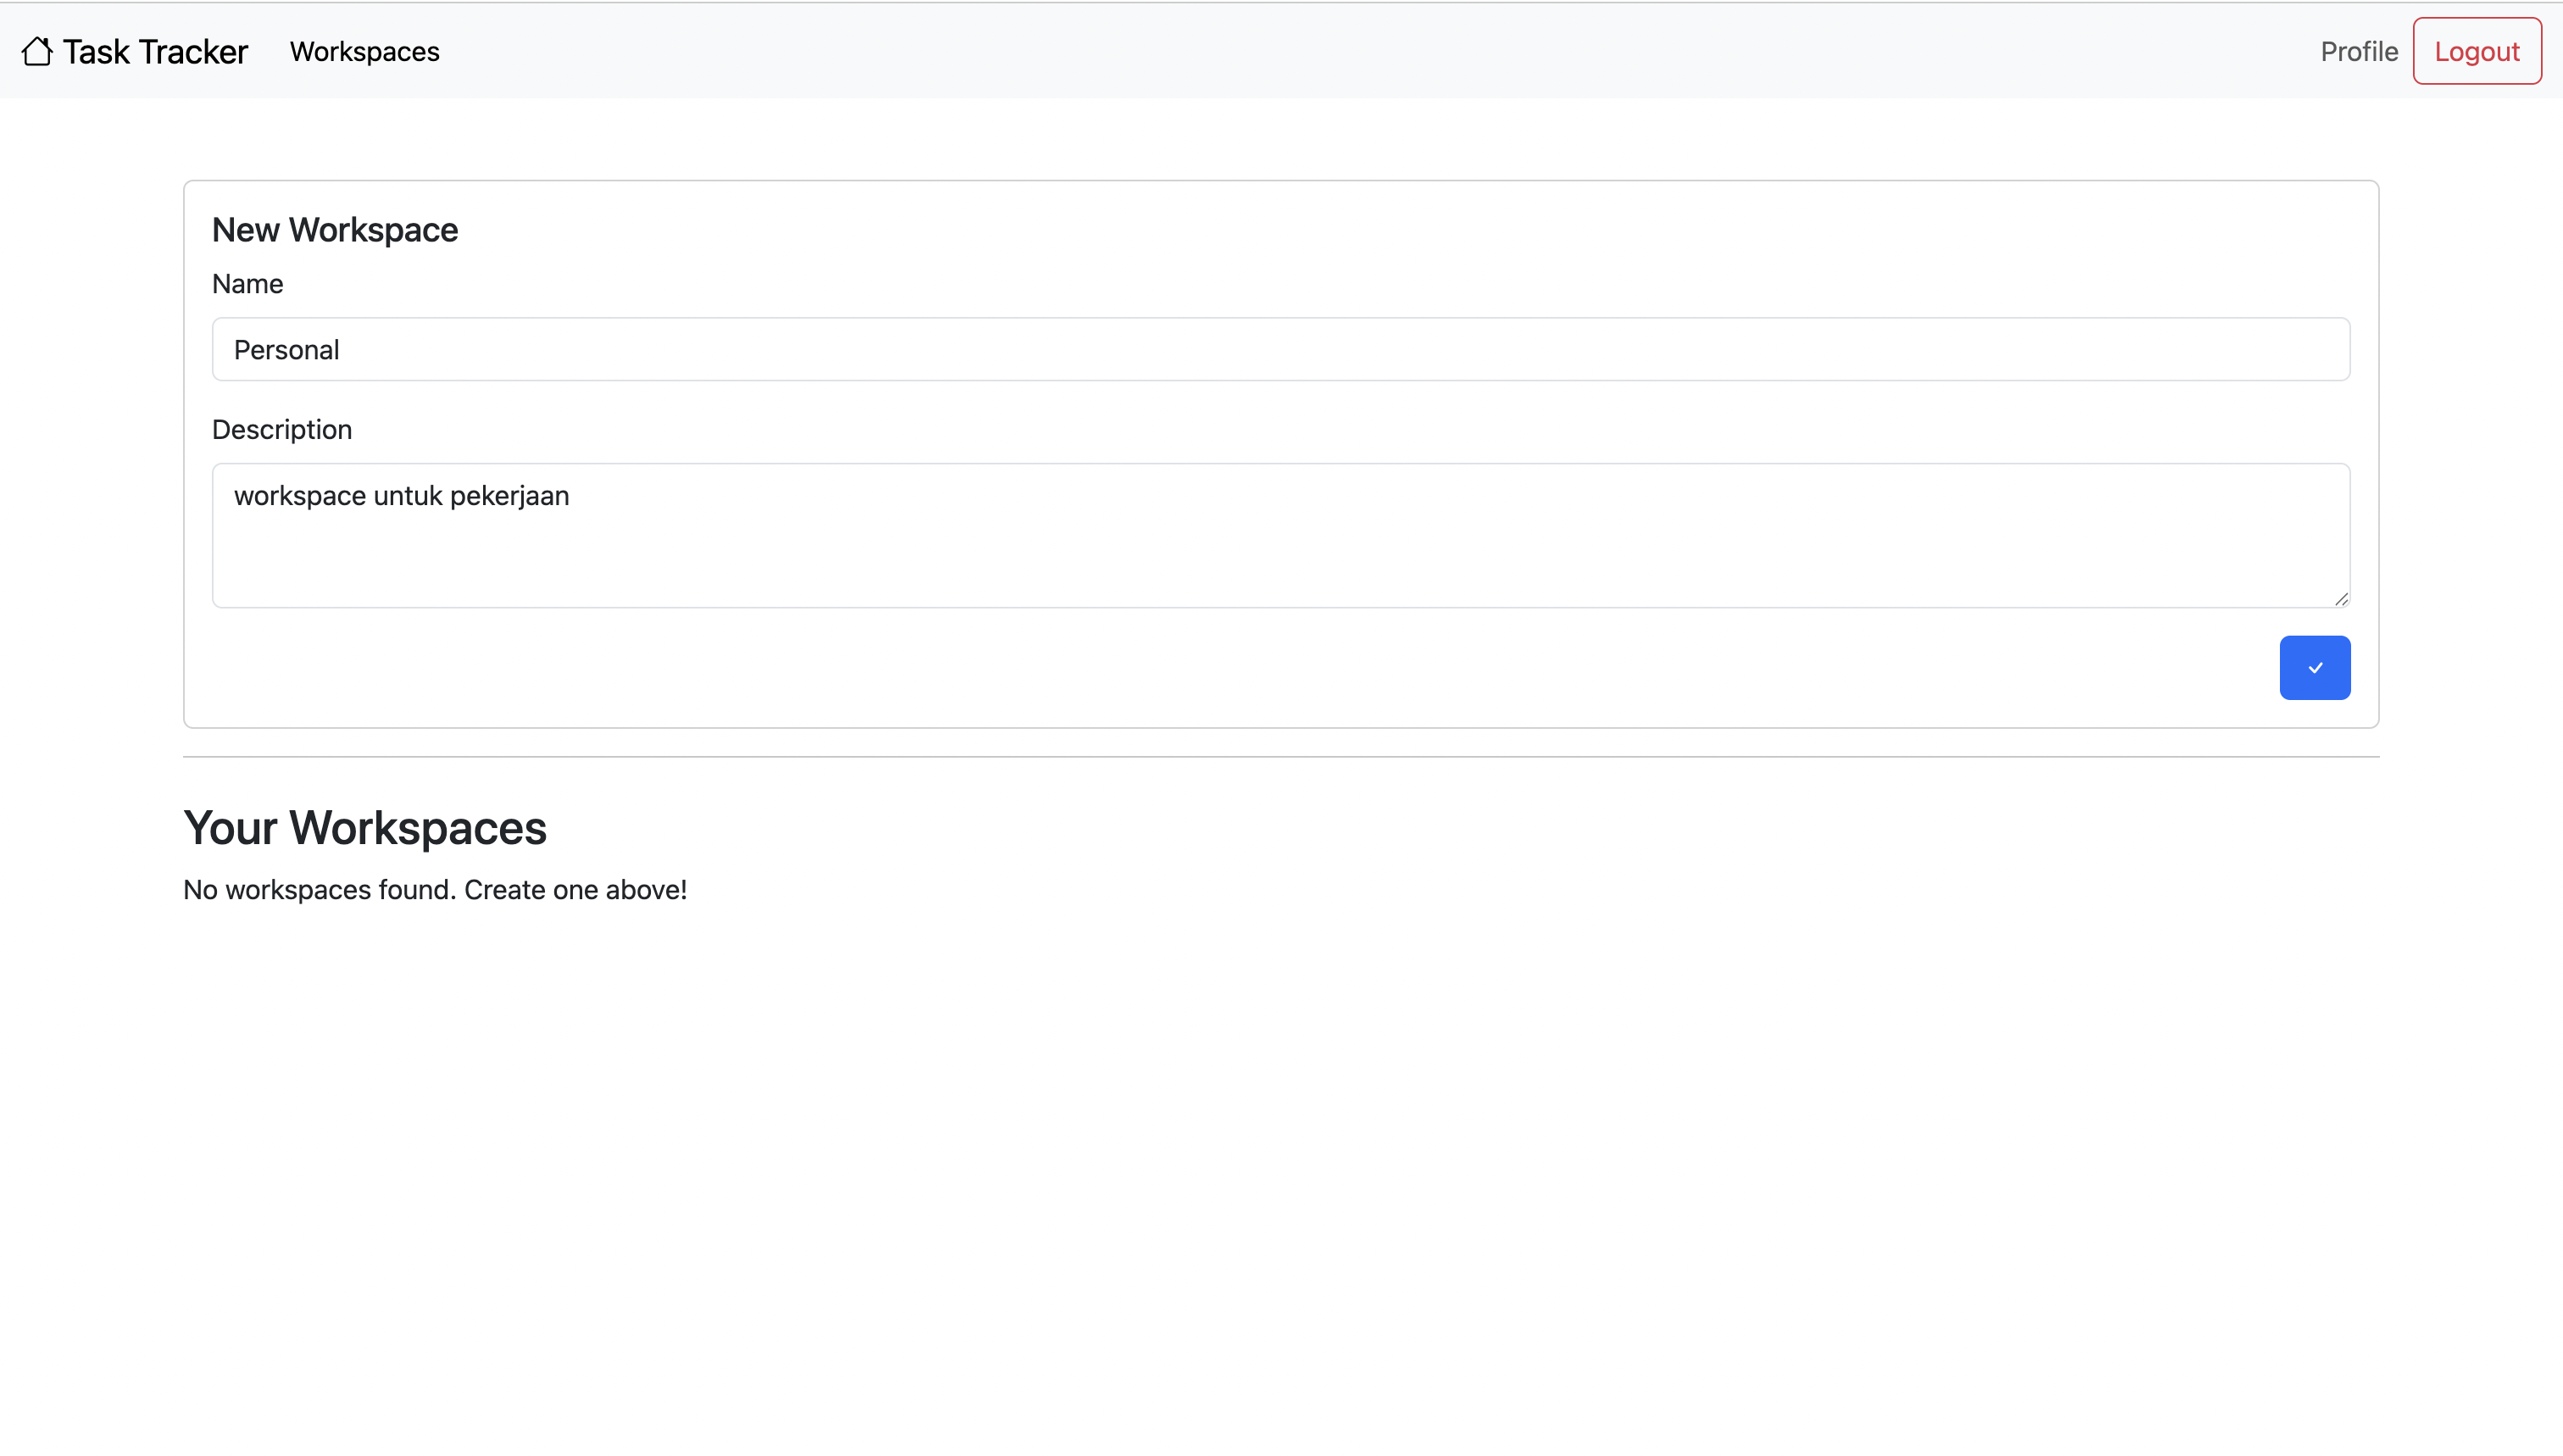
\includegraphics[width=1\textwidth]{assets/ui/workspace_create_filled.png}
  \captionof{figure}{Tampilan UI Workspace dengan Form Create Workspace Terisi}
\end{center}
\begin{center}
  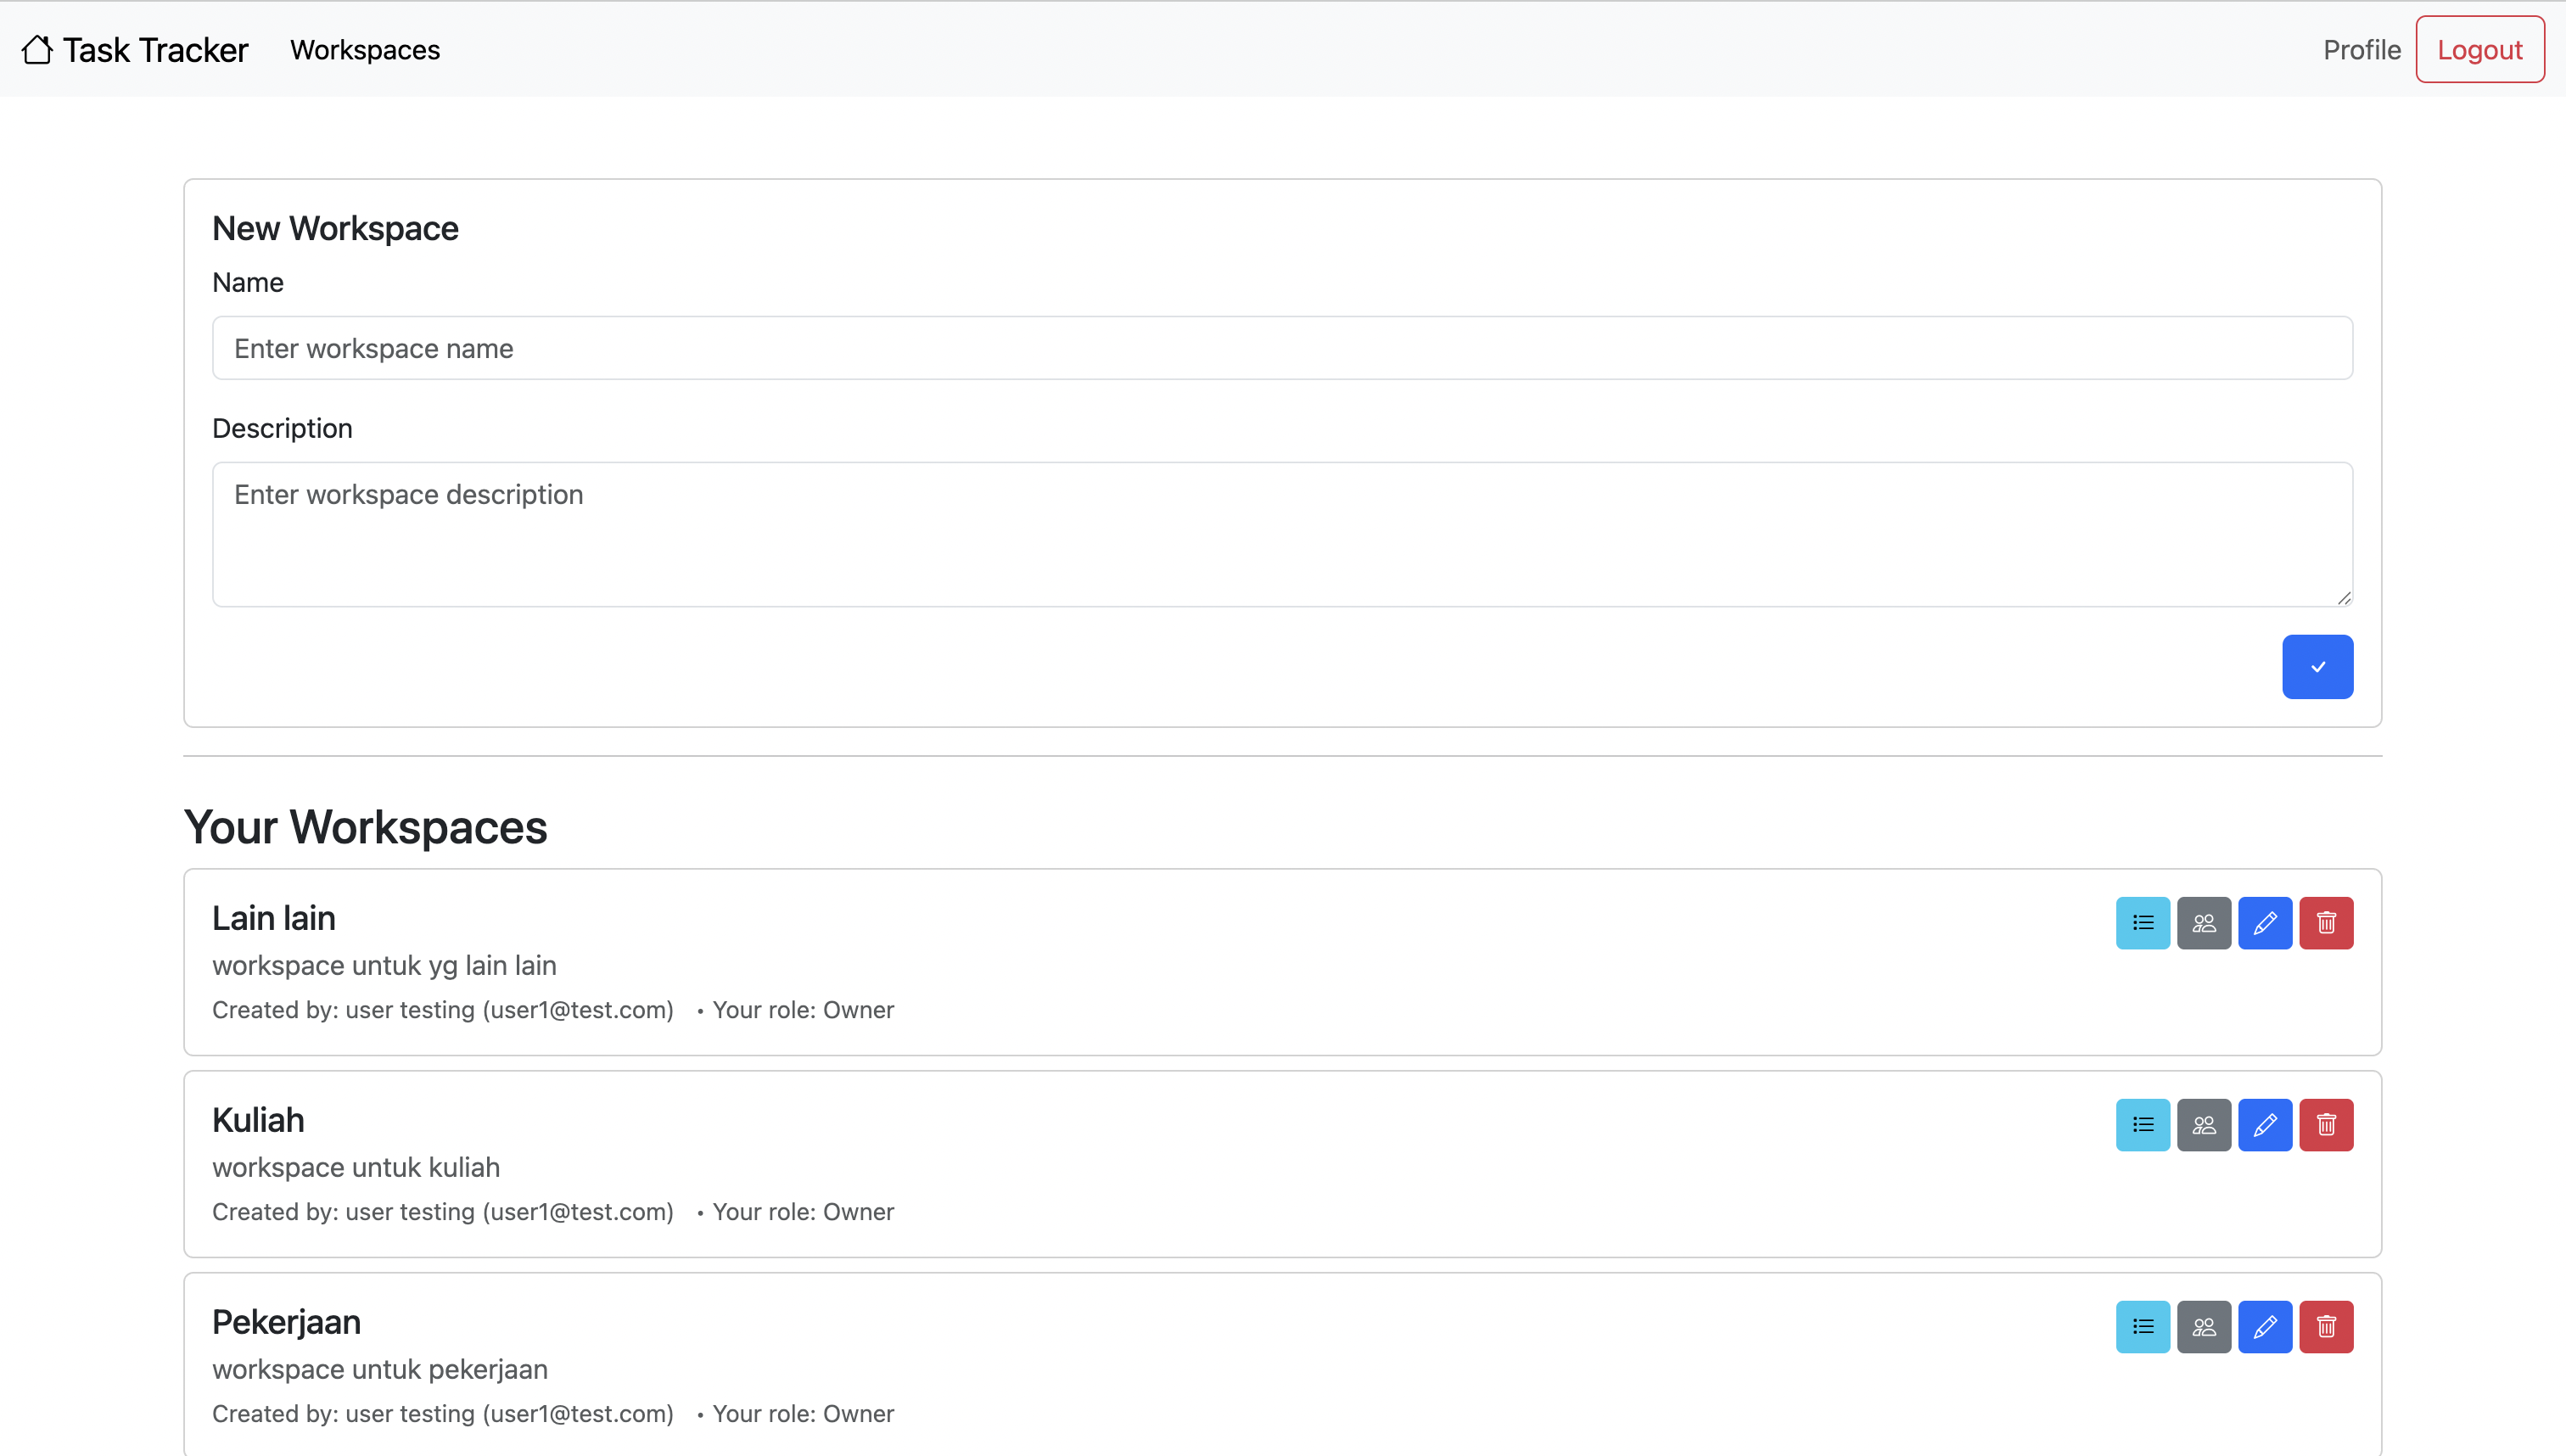
\includegraphics[width=1\textwidth]{assets/ui/list_workspace.png}
  \captionof{figure}{Tampilan UI List Workspace}
\end{center}
\begin{center}
  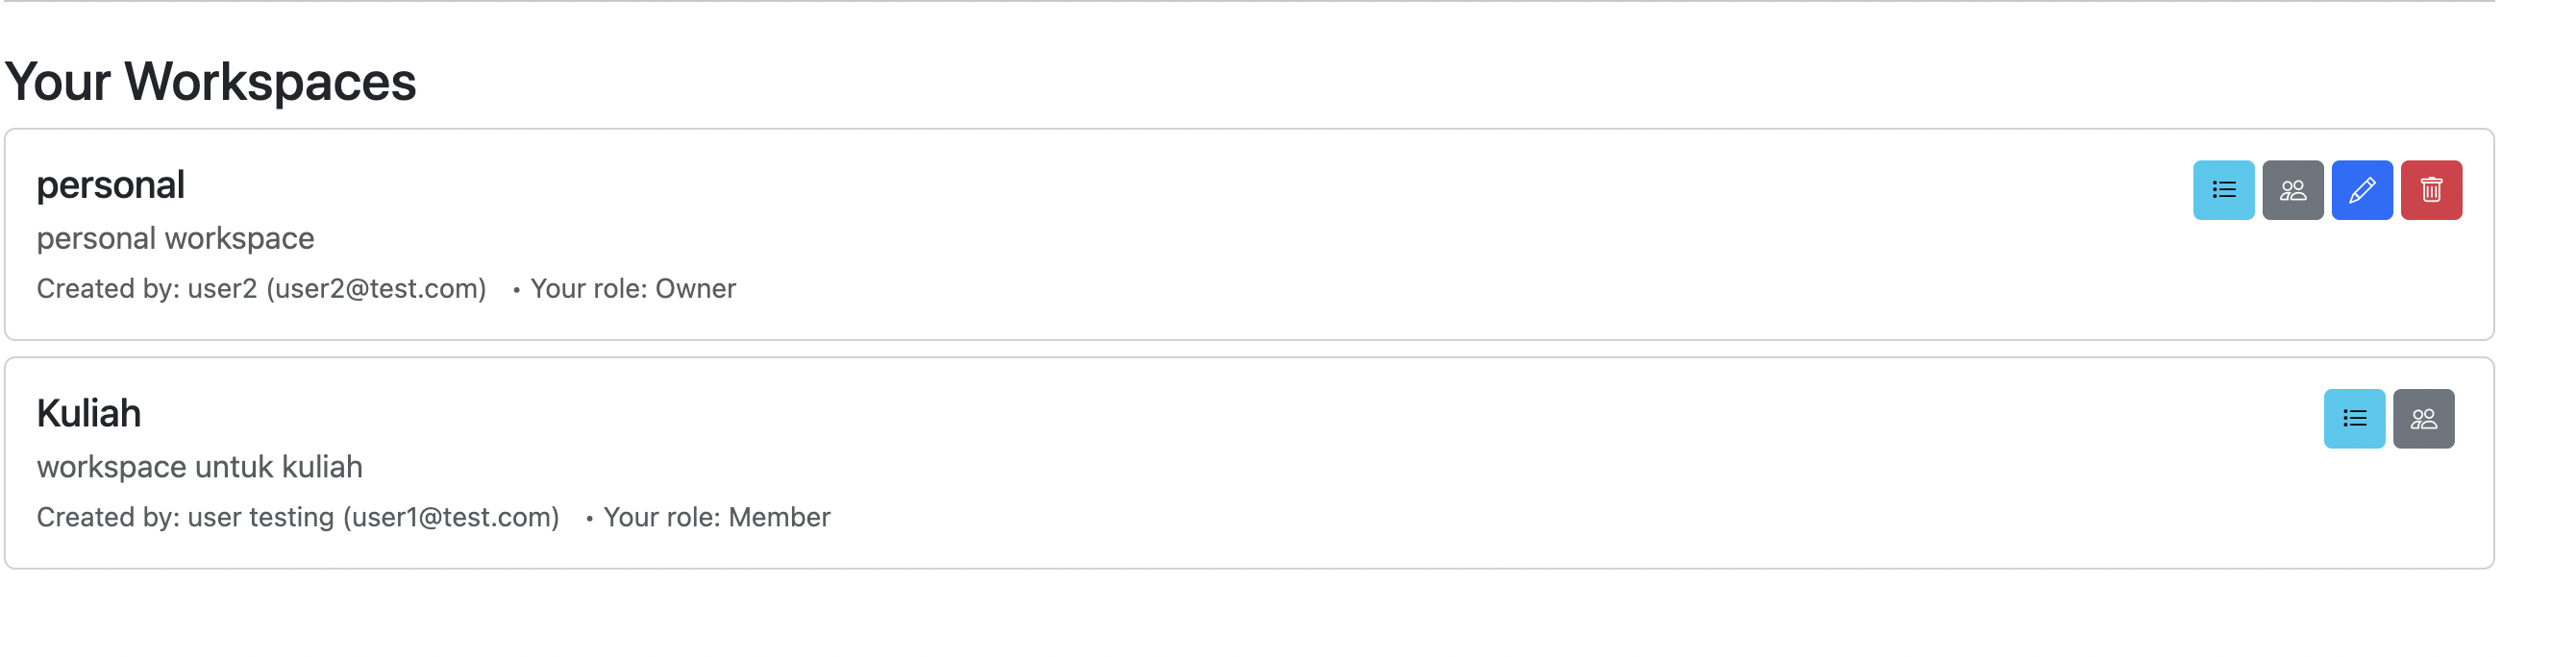
\includegraphics[width=1\textwidth]{assets/ui/workspace_list_row.png}
  \captionof{figure}{Detail UI Item List Workspace}
\end{center}

\subsection*{4.2.6 Tampilan UI Member}
halaman member digunakan untuk manajemen member pada workspace.
seperti menambahkan member baru, dan menghapus member / meninggalkan workspace.
halaman ini bisa diakses dengan cara mengklik icon member pada list workspace.
\begin{center}
  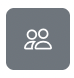
\includegraphics[width=0.1\textwidth]{assets/ui/workspace_member_icon.png}
  \captionof{figure}{Tampilan Icon Member}
\end{center}
\begin{center}
  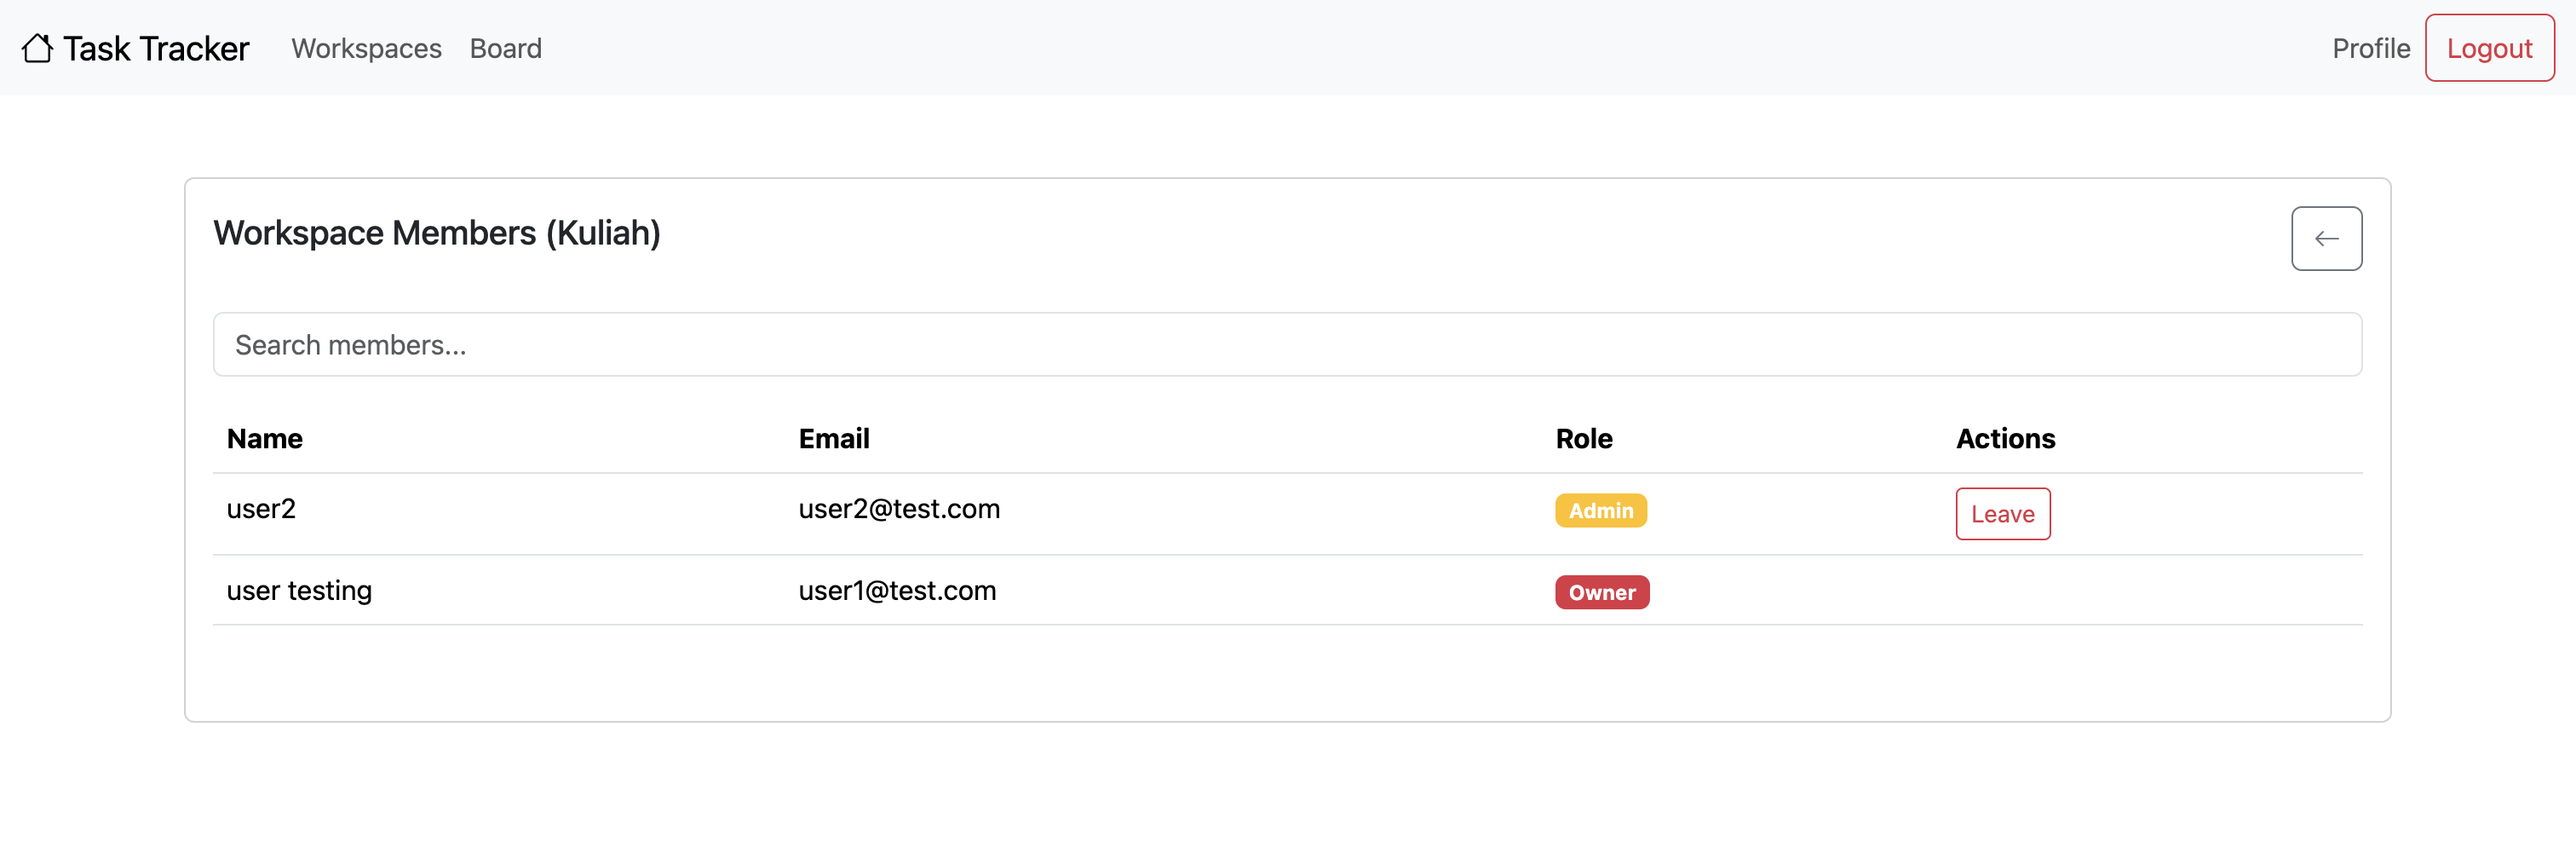
\includegraphics[width=1\textwidth]{assets/ui/list_member.png}
  \captionof{figure}{Tampilan UI List Member Owner}
\end{center}
\begin{center}
  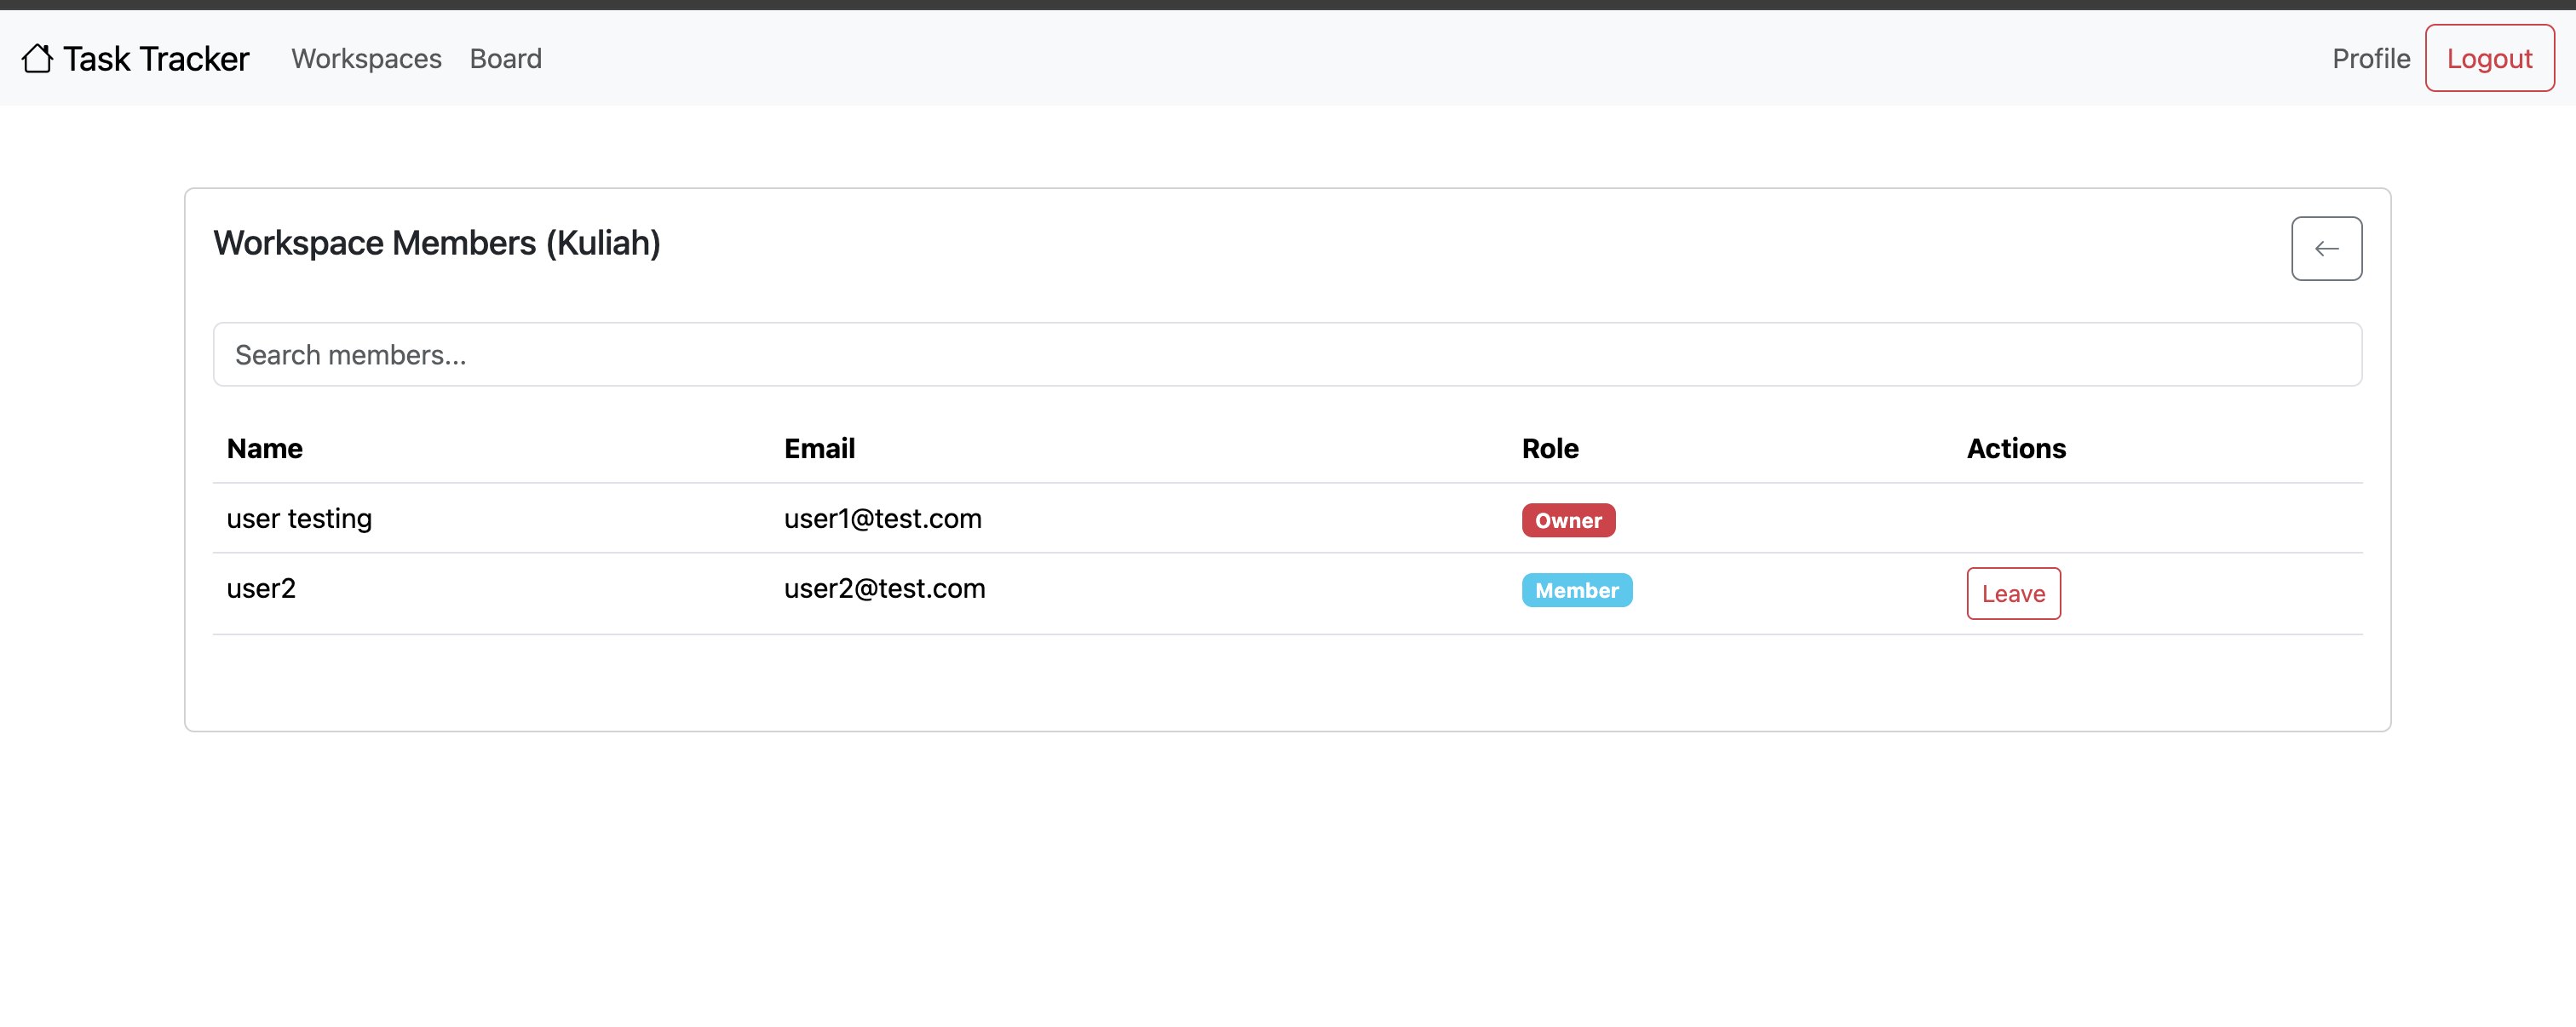
\includegraphics[width=1\textwidth]{assets/ui/list_member_other_user.png}
  \captionof{figure}{Tampilan UI List Member Biasa}
\end{center}










\subsection*{4.2.7 Tampilan UI Task}
